\documentclass[11pt,a4paper]{article}
\usepackage[margin=1.8cm,top=2.5cm,bottom=2.2cm,headheight=24pt]{geometry}
\usepackage{fontspec}
% Preferred font: RakutenSerifApp (author's machine). If it is not found, fall back to TeX Gyre Pagella so the guide compiles anywhere.
\IfFileExists{/home/sudheesh/.fonts/Notesnook/RakutenSerifApp-Regular.ttf}{%
  \setmainfont{RakutenSerifApp}[
    Path = /home/sudheesh/.fonts/Notesnook/,
    Extension = .ttf,
    UprightFont = *-Regular,
    BoldFont = *-Bold,
    ItalicFont = *-Italic,
    BoldItalicFont = *-BoldItalic
  ]%
}{%
  \setmainfont{TeX Gyre Pagella}%
}
\usepackage{amsmath,amssymb,mathtools}
\usepackage{booktabs,array,tabularx,multirow}
\usepackage{graphicx}
\graphicspath{{figures_mod3/}}
\usepackage{xcolor}
\usepackage{titlesec}
\usepackage{fancyhdr}
\usepackage{enumitem}
\usepackage{caption}
\usepackage{tcolorbox}
\tcbuselibrary{skins,breakable}
\usepackage{tikz}
\usepackage{pgfplots}
\pgfplotsset{compat=1.18}
\usetikzlibrary{arrows.meta,calc,positioning,patterns,decorations.pathmorphing}
\usepackage[american]{circuitikz}
% ---- circuit helper macros (switch with anti-parallel diode, capacitor, cell, impedance box) ----
\newcommand{\swleg}[4]{% x, y(centre), switch label, diode label
  \draw[thick] (#1,#2+0.75)--(#1,#2+0.35) (#1,#2-0.35)--(#1,#2-0.75);
  \draw[thick,fill=white] (#1-0.3,#2-0.35) rectangle (#1+0.3,#2+0.35);
  \node[font=\footnotesize] at (#1,#2) {#3};
  \draw[thick] (#1,#2+0.55)--(#1+0.75,#2+0.55)--(#1+0.75,#2+0.2) (#1+0.75,#2-0.2)--(#1+0.75,#2-0.55)--(#1,#2-0.55);
  \draw[thick,fill=black] (#1+0.63,#2-0.2)--(#1+0.87,#2-0.2)--(#1+0.75,#2+0.2)--cycle;
  \draw[thick] (#1+0.63,#2+0.2)--(#1+0.87,#2+0.2);
  \node[font=\scriptsize,right] at (#1+0.88,#2) {#4};
}
\newcommand{\capplate}[2]{\fill[white] (#1-0.3,#2-0.14) rectangle (#1+0.3,#2+0.14);\draw[thick] (#1-0.28,#2+0.1)--(#1+0.28,#2+0.1) (#1-0.28,#2-0.1)--(#1+0.28,#2-0.1);}
\newcommand{\cellplate}[2]{\fill[white] (#1-0.3,#2-0.2) rectangle (#1+0.3,#2+0.2);\draw[thick] (#1-0.3,#2+0.1)--(#1+0.3,#2+0.1) (#1-0.16,#2-0.1)--(#1+0.16,#2-0.1);}
\newcommand{\dn}[3]{% x, y(top), label : downward-conducting series diode
  \draw[thick,fill=black] (#1-0.17,#2)--(#1+0.17,#2)--(#1,#2-0.35)--cycle; \draw[thick] (#1-0.17,#2-0.35)--(#1+0.17,#2-0.35); \node[font=\scriptsize,right] at (#1+0.22,#2-0.17) {#3};}
\newcommand{\sbx}[3]{\draw[thick,fill=white] (#1-0.32,#2-0.3) rectangle (#1+0.32,#2+0.3); \node[font=\footnotesize] at (#1,#2) {#3};}
\newcommand{\zbox}[4]{\draw[thick,fill=white] (#1-#3/2,#2-0.2) rectangle (#1+#3/2,#2+0.2); \node[font=\scriptsize] at (#1,#2) {#4};}
\usepackage[hidelinks,pdfusetitle]{hyperref}

% Define custom column for tabularx
\newcolumntype{Y}{>{\centering\arraybackslash}X}

% Define color palette
\definecolor{navyprimary}{RGB}{15, 35, 65}
\definecolor{accentblue}{RGB}{2, 132, 199}
\definecolor{tealaccent}{RGB}{13, 148, 136}
\definecolor{cardbg}{RGB}{248, 250, 252}
\definecolor{cardborder}{RGB}{203, 213, 225}
\definecolor{calloutbg}{RGB}{241, 245, 249}
\definecolor{calloutframe}{RGB}{100, 116, 139}
\definecolor{formulabg}{RGB}{238, 242, 255}
\definecolor{formulaframe}{RGB}{99, 102, 241}
\definecolor{examplebg}{RGB}{250, 250, 250}
\definecolor{exampleframe}{RGB}{56, 189, 248}
\definecolor{highlightgold}{RGB}{180, 83, 9}
\definecolor{alertbg}{RGB}{254, 242, 242}
\definecolor{alertframe}{RGB}{239, 68, 68}

% Caption styling
\captionsetup{font=small,labelfont={bf,color=navyprimary},skip=5pt}

% Typography & Header/Footer
\pagestyle{fancy}
\fancyhf{}
\renewcommand{\headrulewidth}{0.6pt}
\renewcommand{\headrule}{\hbox to\headwidth{\color{navyprimary}\leaders\hrule height \headrulewidth\hfill}}
\fancyhead[L]{\small\bfseries\color{navyprimary}Power Electronics (Module 3) --- Master Study Guide}
\fancyhead[R]{\small\color{accentblue}CET S5 EEE}
\fancyfoot[L]{\small\color{gray}College of Engineering Trivandrum}
\fancyfoot[R]{\small\bfseries\color{navyprimary}Page \thepage}

% Section Titles Styling
\titleformat{\section}{\Large\bfseries\color{navyprimary}}{}{0em}{}[\vspace{1mm}{\color{accentblue}\hrule height 1.2pt}]
\titleformat{\subsection}{\large\bfseries\color{accentblue}}{}{0em}{}
\titleformat{\subsubsection}{\normalsize\bfseries\color{tealaccent}}{}{0em}{}
% keep headings together with the text that follows them (avoids a heading stranded at the bottom of a page)
\usepackage{needspace}
\let\origsection\section
\renewcommand{\section}{\Needspace{12\baselineskip}\origsection}
\let\origsubsection\subsection
\renewcommand{\subsection}{\Needspace{7\baselineskip}\origsubsection}

% Tcolorbox custom environments (Border-free modern cards with solid background colors)
\newtcolorbox{conceptbox}[1][]{
  enhanced,
  colback=calloutbg,
  colframe=calloutbg,
  colbacktitle=calloutbg,
  coltitle=navyprimary,
  fonttitle=\bfseries,
  title={#1},
  titlerule=0pt,
  boxrule=0pt,
  frame hidden,
  arc=2.5mm,
  left=4mm, right=4mm, top=3mm, bottom=3mm,
  breakable
}

\newtcolorbox{formulabox}[1][]{
  enhanced,
  colback=formulabg,
  colframe=formulabg,
  colbacktitle=formulabg,
  coltitle=navyprimary,
  fonttitle=\bfseries,
  title={#1},
  titlerule=0pt,
  boxrule=0pt,
  frame hidden,
  arc=2.5mm,
  left=4mm, right=4mm, top=3mm, bottom=3mm,
  breakable
}

\newtcolorbox{examplebox}[1][]{
  enhanced,
  colback=examplebg,
  colframe=examplebg,
  colbacktitle=examplebg,
  coltitle=navyprimary,
  fonttitle=\bfseries,
  title={#1},
  titlerule=0pt,
  boxrule=0pt,
  frame hidden,
  arc=2.5mm,
  left=4mm, right=4mm, top=3mm, bottom=3mm,
  middle=2.5mm,
  segmentation style={solid, draw=cardborder, line width=0.6pt},
  breakable
}

\newtcolorbox{alertbox}[1][]{
  enhanced,
  colback=alertbg,
  colframe=alertbg,
  colbacktitle=alertbg,
  coltitle=alertframe,
  fonttitle=\bfseries,
  title={#1},
  titlerule=0pt,
  boxrule=0pt,
  frame hidden,
  arc=2.5mm,
  left=4mm, right=4mm, top=3mm, bottom=3mm,
  breakable
}

% Remove boxed black borders
\renewcommand{\boxed}[1]{#1}

\begin{document}

% Title Block
\begin{center}
  {\LARGE\bfseries\color{navyprimary}POWER ELECTRONICS}\\[2mm]
  {\Large\bfseries\color{accentblue}Module 3: AC Voltage Controllers, DC-AC Inverters \& Utility Interface}\\[3mm]
  {\normalsize\bfseries B.Tech S5 Electrical \& Electronics Engineering (EEE) $\cdot$ APJ Abdul Kalam Technological University}\\[1mm]
  {\small\color{gray}Comprehensive Master Study Guide \& University Examination Preparation Manual}\\[1mm]
  {\footnotesize\color{gray}Revised edition --- equations re-derived, worked problems re-computed numerically, figures redrawn}\\[2mm]
  \noindent\makebox[\linewidth]{\color{navyprimary}\rule{\linewidth}{1.5pt}}
\end{center}

\vspace{-2mm}
\tableofcontents
\vspace{4mm}
\noindent\makebox[\linewidth]{\color{cardborder}\rule{\linewidth}{0.6pt}}
\vspace{2mm}

\section{AC Voltage Controllers (ACVC) / AC Regulators}

\subsection{Foundational Principles and Classification}

An \textbf{AC Voltage Controller} (also termed an \textbf{AC Voltage Regulator}) is a line-frequency phase-controlled or integral-cycle switched converter that converts a fixed-voltage, fixed-frequency alternating current supply into a \textbf{variable-voltage, fixed-frequency AC output} without an intermediate DC stage:
\begin{equation}
\text{Fixed AC Input } (V_s, f) \xrightarrow{\text{AC Voltage Controller}} \text{Variable AC Output } (V_{or}, f)
\end{equation}
Because conversion is accomplished entirely in a single stage using line-commutated thyristors or TRIACs, AC voltage controllers feature extremely high operational efficiency ($\eta > 98\%$), rugged mechanical simplicity, low initial cost, and the complete absence of bulky reactive filter banks.

\subsubsection{Classification of AC Voltage Control Methods}
AC voltage controllers are categorized into three distinct operational methodologies according to the switching mechanism employed (frequently evaluated in university examinations):

\begin{enumerate}[leftmargin=*]
  \item \textbf{Phase Angle Control (PAC):}
  \begin{itemize}[leftmargin=*]
    \item \textbf{Mechanism:} The power semiconductor switches (a pair of anti-parallel SCRs or a TRIAC) connect the load to the AC source for a controllable fraction of each supply half-cycle. Conduction is initiated at a controllable delay angle $\alpha$ (measured relative to the zero-crossing of the input supply voltage) and ceases naturally at current zero ($\beta$) via natural (line) commutation.
    \item \textbf{Advantages:} Provides continuous, smooth, instantaneous, and infinitely variable control of RMS load voltage from $0$ to $V_s$.
    \item \textbf{Disadvantages:} The abrupt chopping of sinusoidal voltage waveforms introduces substantial low-order current harmonics (3rd, 5th, 7th) and causes the supply displacement factor to lag significantly as $\alpha$ increases.
    \item \textbf{Primary Applications:} Universal motor speed control, light dimmers, induction motor soft-starters, industrial furnace heating.
  \end{itemize}

  \item \textbf{Integral Cycle Control (On-Off / Burst Firing Control):}
  \begin{itemize}[leftmargin=*]
    \item \textbf{Mechanism:} The thyristor switches connect the load to the AC mains for an integral number of complete supply cycles ($n$ cycles), and then remain un-triggered for another integral number of cycles ($m$ cycles). Switching is always synchronized to occur at the zero-crossing of the supply voltage ($v_s(t) = 0$).
    \item \textbf{Mathematical Duty Ratio and RMS Voltage:}
    \begin{equation}
    k = \frac{n}{n + m} = \frac{T_{on}}{T_o} \implies V_{or} = V_s \sqrt{k} = V_s \sqrt{\frac{n}{n + m}}
    \end{equation}
    where $T_o = (n + m)T$ is the overall repeating period.
    \item \textbf{Advantages:} Because switching transitions occur exclusively at natural voltage zero-crossings ($dv/dt \to 0$ and $di/dt \to 0$), radio frequency interference (RFI), electromagnetic interference (EMI), and switching losses are virtually zero.
    \item \textbf{Disadvantages:} Sub-harmonic frequency components (frequencies below the mains supply frequency $f$) and line flicker are introduced, making this method completely unsuitable for motor speed control or lighting systems.
    \item \textbf{Primary Applications:} Loads with very large mechanical or thermal time constants, such as industrial electric ovens, boiler heaters, and plastic extrusion mold heaters.
  \end{itemize}

  \item \textbf{Sequence Control of AC Voltage Controllers:}
  \begin{itemize}[leftmargin=*]
    \item \textbf{Mechanism:} Two or more parallel transformer-tapped stages of AC voltage controllers are fired in sequence. By controlling only one stage at a time while leaving others fully ON or fully OFF, the output voltage is varied with substantially reduced harmonic distortion and a significantly improved supply power factor across the entire operating range.
  \end{itemize}
\end{enumerate}

\begin{figure}[htbp]
\centering
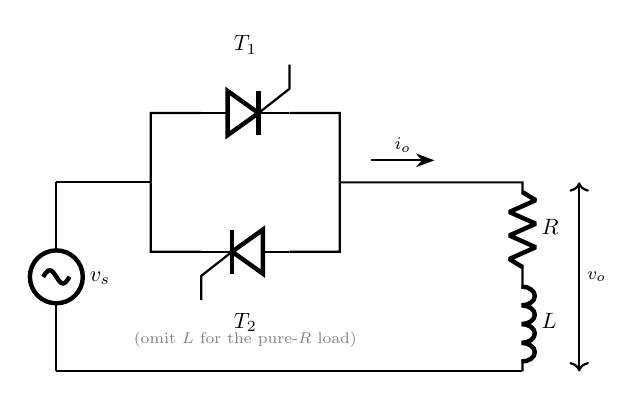
\begin{tikzpicture}[thick,scale=0.8,transform shape]
 \draw (0,0) to[sinusoidal voltage source, l_=$v_s$] (0,3);
 \draw (0,3)--(1.5,3) (0,0)--(7.4,0);
 \draw (1.5,3)--(1.5,4.1) to[thyristor, l=$T_1$] (4.5,4.1)--(4.5,3);
 \draw (4.5,3)--(4.5,1.9) to[thyristor, l=$T_2$] (1.5,1.9)--(1.5,3);
 \draw (4.5,3)--(7.4,3) to[R, l=$R$] (7.4,1.5) to[L, l=$L$] (7.4,0);
 \draw[-{Stealth}] (5.0,3.35)--(6.0,3.35) node[midway,above,font=\footnotesize]{$i_o$};
 \draw[<->] (8.3,3)--(8.3,0) node[midway,right,font=\footnotesize]{$v_o$};
 \node[font=\scriptsize,gray] at (3,0.5) {(omit $L$ for the pure-$R$ load)};
\end{tikzpicture}
\\[3mm]
\includegraphics[width=0.72\textwidth]{fig_acvc_r.pdf}
\caption{Single-phase full-wave AC voltage controller with resistive load, $\alpha=60^\circ$: (a) power circuit with two anti-parallel thyristors $T_1$, $T_2$ (add the series inductance $L$ for the $RL$ case); (b) waveforms of supply and load voltage, gate pulses, load current $i_o=v_o/R$ and the voltage $v_T$ across the thyristor pair. (Redrawn; compare Hart Fig.~5-1.)}
\label{fig:acvc_r_circuit}
\end{figure}

\subsection{Single-Phase Full-Wave AC Voltage Controller with Pure Resistive ($R$) Load}

Consider the circuit of Figure~\ref{fig:acvc_r_circuit}a supplied by a single-phase sinusoidal AC source $v_s(t) = V_m \sin(\omega t) = \sqrt{2}V_s \sin(\omega t)$. Two SCRs ($T_1$ and $T_2$) are connected in anti-parallel (back-to-back) between the AC mains and a resistive load $R$.

\subsubsection{Circuit Operation Across One Full Fundamental Cycle}
\begin{itemize}[leftmargin=*]
  \item \textbf{Positive Half-Cycle ($0 \le \omega t \le \pi$):} Supply voltage $v_s > 0$. Thyristor $T_1$ is forward-biased, while $T_2$ is reverse-biased ($v_{AK2} < 0$).
  \begin{itemize}
    \item From $\omega t = 0$ to $\omega t = \alpha$, $T_1$ remains OFF. No current flows ($i_o = 0$), load voltage $v_o = 0$, and the full line voltage appears across $T_1$ ($v_{T1} = v_s$).
    \item At $\omega t = \alpha$, a firing pulse is applied to the gate of $T_1$. $T_1$ turns ON instantaneously.
    \item From $\omega t = \alpha$ to $\pi$, $T_1$ conducts load current:
    \begin{equation}
    v_o(t) = v_s(t) = V_m \sin(\omega t), \quad i_o(t) = \frac{v_s(t)}{R} = \frac{V_m}{R}\sin(\omega t)
    \end{equation}
    \item At $\omega t = \pi$, the supply voltage reverses polarity. The current through $T_1$ drops naturally to zero ($i_o(\pi) = 0$), turning $T_1$ OFF via natural (line) commutation.
  \end{itemize}

  \item \textbf{Negative Half-Cycle ($\pi \le \omega t \le 2\pi$):} Supply voltage $v_s < 0$. Thyristor $T_2$ is forward-biased, while $T_1$ is reverse-biased.
  \begin{itemize}
    \item At $\omega t = \pi + \alpha$, a firing pulse is applied to the gate of $T_2$. $T_2$ turns ON.
    \item From $\omega t = \pi + \alpha$ to $2\pi$, $T_2$ conducts negative load current:
    \begin{equation}
    v_o(t) = v_s(t) = V_m \sin(\omega t), \quad i_o(t) = \frac{V_m}{R}\sin(\omega t) \quad (< 0)
    \end{equation}
    \item At $\omega t = 2\pi$, $i_o(2\pi) = 0$, and $T_2$ turns OFF naturally.
  \end{itemize}
\end{itemize}

\subsubsection{Rigorous Mathematical Derivation of RMS Output Voltage}
Because the output voltage waveform exhibits half-wave symmetry ($v_o(\omega t + \pi) = -v_o(\omega t)$), the root-mean-square (RMS) value can be computed over a half-cycle ($0$ to $\pi$):
\begin{align}
V_{or} &= \sqrt{\frac{1}{\pi} \int_{\alpha}^{\pi} \left[V_m \sin(\omega t)\right]^2 d(\omega t)} = \sqrt{\frac{V_m^2}{\pi} \int_{\alpha}^{\pi} \frac{1 - \cos(2\omega t)}{2} d(\omega t)} \notag\\
&= \sqrt{\frac{V_m^2}{2\pi} \left[ \omega t - \frac{\sin(2\omega t)}{2} \right]_{\alpha}^{\pi}} = \sqrt{\frac{V_m^2}{2\pi} \left[ (\pi - \alpha) - \left(\frac{\sin(2\pi) - \sin(2\alpha)}{2}\right) \right]} \notag\\
&= \sqrt{\frac{V_m^2}{2\pi} \left[ (\pi - \alpha) + \frac{\sin(2\alpha)}{2} \right]} = \frac{V_m}{\sqrt{2}} \sqrt{\frac{1}{\pi} \left[ (\pi - \alpha) + \frac{\sin(2\alpha)}{2} \right]}
\end{align}
Recognizing that $V_s = V_m / \sqrt{2}$ is the RMS value of the input source:
\begin{formulabox}[Master Equation: RMS Output Voltage ($R$ Load)]
\begin{equation}
V_{or} = V_s \sqrt{1 - \frac{\alpha}{\pi} + \frac{\sin(2\alpha)}{2\pi}}
\label{eq:acvc_rms_r}
\end{equation}
\end{formulabox}

\subsubsection{Performance Characteristics with $R$ Load}
\begin{itemize}[leftmargin=*]
  \item \textbf{RMS Load Current:} $I_{or} = \frac{V_{or}}{R} = \frac{V_s}{R} \sqrt{1 - \frac{\alpha}{\pi} + \frac{\sin(2\alpha)}{2\pi}}$.
  \item \textbf{Average and RMS Thyristor Currents:} Each thyristor conducts for only one half of the symmetrical period:
  \begin{equation}
  I_{T(avg)} = \frac{1}{2\pi} \int_{\alpha}^{\pi} \frac{V_m}{R}\sin(\omega t) d(\omega t) = \frac{V_m}{2\pi R} (1 + \cos\alpha) = \frac{\sqrt{2}V_s}{2\pi R}(1 + \cos\alpha)
  \end{equation}
  \begin{equation}
  I_{T(rms)} = \frac{I_{or}}{\sqrt{2}} = \frac{V_s}{\sqrt{2}R} \sqrt{1 - \frac{\alpha}{\pi} + \frac{\sin(2\alpha)}{2\pi}}
  \end{equation}
  \item \textbf{Input Power Factor (PF):} Since input current $i_s(t) = i_o(t)$, the apparent power supplied by the mains is $S = V_s I_{or}$. The active power dissipated in the load is $P_o = I_{or}^2 R = \frac{V_{or}^2}{R}$.
  \begin{equation}
  \text{PF} = \frac{P_o}{S} = \frac{V_{or}^2 / R}{V_s I_{or}} = \frac{V_{or} I_{or}}{V_s I_{or}} = \frac{V_{or}}{V_s} = \sqrt{1 - \frac{\alpha}{\pi} + \frac{\sin(2\alpha)}{2\pi}}
  \end{equation}
  \item \textbf{Control Range:} As $\alpha$ varies from $0$ to $\pi$ ($180^\circ$):
  \begin{itemize}
    \item At $\alpha = 0$: $V_{or} = V_s$, $\text{PF} = 1.0$ (Full sinusoidal conduction).
    \item At $\alpha = \pi/2$ ($90^\circ$): $V_{or} = V_s / \sqrt{2} \approx 0.707 V_s$, $\text{PF} \approx 0.707$.
    \item At $\alpha = \pi$ ($180^\circ$): $V_{or} = 0$, $\text{PF} = 0$ (Output completely blocked).
  \end{itemize}
\end{itemize}

\subsection{Single-Phase Full-Wave AC Voltage Controller with $RL$ Load}

When the load consists of an inductive impedance $Z = \sqrt{R^2 + (\omega L)^2}$ with characteristic load impedance angle $\phi = \arctan\left(\frac{\omega L}{R}\right)$, the inductance opposes sudden changes in load current. Consequently, \textbf{the current continues to flow after the source voltage reverses polarity at $\omega t = \pi$}.

\begin{figure}[htbp]
\centering
\includegraphics[width=0.68\textwidth]{hart_fig_5_4_acvc_rl.png}
\caption{Single-phase AC voltage controller with $RL$ load: (a) circuit; (b) typical waveforms of the supply voltage $v_s$, load current $i_o$, load voltage $v_o$ and switch voltage $v_{sw}$, showing the delay angle $\alpha$, the extinction angle $\beta$ and the instant $\pi+\alpha$ at which $T_2$ is fired. (Source: Daniel W. Hart, Fig.\ 5-4)}
\label{fig:acvc_rl_waveforms}
\end{figure}

\subsubsection{Derivation of the Load Current Differential Equation}
During the conduction of thyristor $T_1$ ($\alpha \le \omega t \le \beta$), the governing Kirchhoff's Voltage Law (KVL) differential equation is:
\begin{equation}
L \frac{di_o(t)}{dt} + R i_o(t) = v_s(t) = V_m \sin(\omega t)
\end{equation}
The total solution consists of a steady-state particular solution $i_{ss}(t)$ and a transient complementary solution $i_{tr}(t)$:
\begin{equation}
i_o(\omega t) = \frac{V_m}{Z}\sin(\omega t - \phi) + A e^{-\frac{R}{\omega L}\omega t}
\end{equation}
where $Z = \sqrt{R^2 + (\omega L)^2}$ and $\phi = \arctan(\omega L / R)$.

Applying the initial boundary condition at the firing instant: at $\omega t = \alpha$, $i_o(\alpha) = 0$:
\begin{equation}
0 = \frac{V_m}{Z}\sin(\alpha - \phi) + A e^{-\frac{R}{\omega L}\alpha} \implies A = -\frac{V_m}{Z}\sin(\alpha - \phi) e^{\frac{R}{\omega L}\alpha}
\end{equation}
Substituting $A$ back into the current expression yields the closed-form equation for the instantaneous load current:
\begin{formulabox}[Instantaneous Load Current in ACVC with $RL$ Load]
\begin{equation}
i_o(\omega t) = \frac{V_m}{Z} \left[ \sin(\omega t - \phi) - \sin(\alpha - \phi) e^{-\frac{R}{\omega L}(\omega t - \alpha)} \right], \quad \text{for } \alpha \le \omega t \le \beta
\label{eq:acvc_io_rl}
\end{equation}
\end{formulabox}

\subsubsection{Extinction Angle ($\beta$) and Conduction Angle ($\gamma$)}
At $\omega t = \beta$, the magnetic energy stored in inductor $L$ is completely dissipated into $R$, and the current extinguishes to zero ($i_o(\beta) = 0$). Setting equation~\eqref{eq:acvc_io_rl} to zero at $\omega t = \beta$ gives the transcendental equation:
\begin{equation}
\sin(\beta - \phi) = \sin(\alpha - \phi) e^{-\frac{R}{\omega L}(\beta - \alpha)}
\label{eq:acvc_beta_transcendental}
\end{equation}
The conduction angle of each thyristor is defined as $\gamma = \beta - \alpha$. Equation~\eqref{eq:acvc_beta_transcendental} can be expressed in terms of $\gamma$ as:
\begin{equation}
\sin(\alpha + \gamma - \phi) = \sin(\alpha - \phi) e^{-\frac{R}{\omega L}\gamma}
\end{equation}

\subsubsection{Three Critical Conduction Regimes Based on Firing Angle $\alpha$ vs $\phi$}
The behavior of the $RL$ AC voltage controller depends decisively on the relative relationship between the firing delay angle $\alpha$ and the load impedance phase angle $\phi$:

\begin{enumerate}[leftmargin=*]
  \item \textbf{Case 1: $\alpha > \phi$ (Discontinuous Conduction Mode --- Standard Operation):}
  \begin{itemize}
    \item The current extinguishes before the next half-cycle thyristor is triggered: $\beta < \pi + \alpha$, which means the conduction angle $\gamma = (\beta - \alpha) < \pi$.
    \item There is a finite zero-current interval between the extinction of $T_1$ and the firing of $T_2$.
    \item The output voltage is fully controllable by varying $\alpha$ between $\phi$ and $\pi$.
  \end{itemize}

  \item \textbf{Case 2: $\alpha = \phi$ (Boundary / Critical Conduction Mode):}
  \begin{itemize}
    \item Substituting $\alpha = \phi$ into equation~\eqref{eq:acvc_beta_transcendental}:
    \begin{equation}
    \sin(\beta - \phi) = \sin(0) \cdot e^{-\frac{R}{\omega L}(\beta - \phi)} = 0 \implies \beta - \phi = \pi \implies \beta = \pi + \phi = \pi + \alpha
    \end{equation}
    \item The conduction angle is exactly $\gamma = \beta - \alpha = \pi$ ($180^\circ$).
    \item Thyristor $T_1$ conducts for exactly $180^\circ$. The moment $T_1$ extinguishes at $\omega t = \pi + \alpha$, thyristor $T_2$ is triggered!
    \item The load current becomes a continuous, perfectly sinusoidal waveform: $i_o(t) = \frac{V_m}{Z}\sin(\omega t - \phi)$. The converter behaves as if the load is directly connected across the AC supply!
  \end{itemize}

  \item \textbf{Case 3: $\alpha < \phi$ (Loss of Control):}
  \begin{itemize}
    \item The solution above would give $\beta > \pi + \alpha$, i.e.\ $T_1$ would still be carrying current when $T_2$ is gated at $\pi + \alpha$. $T_2$ is then still reverse-biased (the voltage across it is $\approx 0$ while $T_1$ conducts).
    \item \textbf{Long gate pulse:} $T_2$ simply takes over when $T_1$ current reaches zero, i.e.\ at $\omega t = \pi + \phi$. The firing is effectively delayed to $\phi$, the load current is the continuous sinusoid $i_o = \frac{V_m}{Z}\sin(\omega t - \phi)$ and $V_{or} = V_s$ for \emph{every} $\alpha < \phi$. Firing earlier gives no extra output.
    \item \textbf{Short (narrow) gate pulse:} the pulse to $T_2$ is gone before $T_1$ stops conducting, so $T_2$ never fires. Only $T_1$ conducts, the current becomes unidirectional with a DC component, and the supply or motor transformer can saturate.
    \item \textbf{Critical Exam Rule:} $\alpha$ must satisfy $\alpha \ge \phi$. The usable control range is $\phi \le \alpha \le \pi$ (with $V_{or}$ falling from $V_s$ at $\alpha=\phi$ to $0$ at $\alpha=\pi$).
  \end{itemize}
\end{enumerate}

\subsubsection{Derivation of RMS Output Voltage with $RL$ Load}
During the conduction interval $\alpha \le \omega t \le \beta$, the load voltage equals the supply voltage: $v_o(t) = V_m \sin(\omega t)$. Outside this interval, $v_o(t) = 0$.
\begin{align}
V_{or} &= \sqrt{\frac{1}{\pi} \int_{\alpha}^{\beta} \left[V_m \sin(\omega t)\right]^2 d(\omega t)} = \sqrt{\frac{V_m^2}{2\pi} \int_{\alpha}^{\beta} \left[1 - \cos(2\omega t)\right] d(\omega t)} \notag\\
&= \sqrt{\frac{V_m^2}{2\pi} \left[ (\beta - \alpha) - \frac{\sin(2\beta) - \sin(2\alpha)}{2} \right]}
\end{align}
In terms of $V_s = V_m / \sqrt{2}$ and conduction angle $\gamma = \beta - \alpha$:
\begin{formulabox}[Master Equation: RMS Output Voltage ($RL$ Load)]
\begin{equation}
V_{or} = V_s \sqrt{\frac{1}{\pi} \left[ (\beta - \alpha) - \frac{\sin(2\beta) - \sin(2\alpha)}{2} \right]} = V_s \sqrt{\frac{1}{\pi} \left[ \gamma - \frac{\sin(2\beta) - \sin(2\alpha)}{2} \right]}
\label{eq:acvc_rms_rl}
\end{equation}
\end{formulabox}

\subsection{Single-Phase AC Voltage Controller with Pure Inductive ($L$) Load}

For a purely inductive load ($R = 0 \implies \phi = 90^\circ = \pi/2$):
\begin{equation}
L \frac{di_o}{dt} = V_m \sin(\omega t) \implies i_o(\omega t) = \frac{V_m}{\omega L} \int_{\alpha}^{\omega t} \sin(\omega t) d(\omega t) = \frac{V_m}{\omega L} (\cos\alpha - \cos\omega t)
\end{equation}
The current extinguishes when $i_o(\beta) = 0$:
\begin{equation}
\cos\alpha - \cos\beta = 0 \implies \beta = 2\pi - \alpha
\end{equation}
The conduction angle is:
\begin{equation}
\gamma = \beta - \alpha = 2\pi - 2\alpha = 2(\pi - \alpha)
\end{equation}
\begin{itemize}[leftmargin=*]
  \item Since $\phi = \pi/2$ ($90^\circ$), the control range for $\alpha$ is restricted to $\pi/2 \le \alpha \le \pi$.
  \item At $\alpha = \pi/2$: $\beta = 2\pi - \pi/2 = 3\pi/2$, $\gamma = \pi$ ($180^\circ$). Current is continuous.
  \item At $\alpha = \pi$: $\beta = \pi$, $\gamma = 0$. No current flows.
  \item This configuration is the fundamental building block of \textbf{Thyristor-Controlled Reactors (TCR)} utilized extensively in static VAR compensators (SVC) on power transmission grids!
\end{itemize}

\subsection{Gate Firing Pulse Requirements for Inductive Loads}
With an inductive load, a standard short gate trigger pulse ($10 - 20\,\mu\text{s}$) cannot ensure reliable thyristor turn-on:
\begin{conceptbox}[Gate Firing Requirements with Inductive Loads]
Because $di/dt = v_s/L$ is restricted by the load inductance, the anode current rises slowly after triggering. If a short gate pulse ends before the anode current crosses the \textbf{latching current} ($I_L$), the thyristor will immediately turn back OFF when the gate pulse is removed!

Furthermore, due to current overlap between consecutive half-cycles, the incoming thyristor may be triggered while the outgoing thyristor is still conducting.

\textbf{Mandatory Solutions:}
\begin{enumerate}
  \item \textbf{Continuous Gate Gating:} Maintain gate current throughout the desired conduction period ($\alpha$ to $\pi$). (Drawback: High average gate power dissipation).
  \item \textbf{High-Frequency Pulse Train Gating (Carrier Frequency Modulation):} Modulate the firing signal with a $10 - 30\text{ kHz}$ pulse train generated by a 555 timer or microcontroller. This reduces gate power dissipation by $>80\%$ while allowing small, compact pulse isolation transformers!
\end{enumerate}
\end{conceptbox}

\subsection{Engineering Applications of AC Voltage Controllers}
\begin{enumerate}[leftmargin=*]
  \item \textbf{Industrial and Domestic Heating:} Closed-loop temperature regulation in resistance furnaces, kilns, soldering stations, and water heaters.
  \item \textbf{Lighting Control (Dimmers):} Theater stage lighting, architectural illumination, and incandescent lamp dimming.
  \item \textbf{AC Motor Soft Starters:} During the starting of high-power three-phase squirrel-cage induction motors, direct-on-line (DOL) starting draws $6 - 8 \times I_{\text{rated}}$, creating severe line voltage dips. By ramping $\alpha$ from $150^\circ$ down to $\phi$, starting current is limited to $2 - 3 \times I_{\text{rated}}$.
  \item \textbf{Speed Control of AC Fan and Pump Motors:} Controlling stator voltage on high-slip single-phase and three-phase induction motors provides stable variable-speed torque for centrifugal fans and water pumps.
  \item \textbf{On-Load Transformer Tap Changers:} Thyristorized tap changers switch transformer winding taps under full load without mechanical arcing, contact wear, or line interruption.
  \item \textbf{Static VAR Compensators (SVC):} Thyristor-Controlled Reactors (TCR) dynamically absorb variable inductive reactive power ($Q$) to stabilize grid voltages.
\end{enumerate}


\section{Single-Phase Switch-Mode DC-AC Voltage Source Inverters (VSI)}

\subsection{Fundamental Operating Principles and Bridge Topologies}

An \textbf{Inverter} is a power electronic converter that transforms direct current (DC) electrical energy into alternating current (AC) electrical energy at a desired, precisely regulated voltage magnitude and frequency:
\begin{equation}
\text{DC Input } (V_{dc}) \xrightarrow{\text{Inverter}} \text{AC Output } (v_o(t), f_o)
\end{equation}
In a \textbf{Voltage Source Inverter (VSI)}, the DC input source is modeled as an ideal voltage source with negligible internal impedance (stiff DC bus supported by a large electrolytic DC-link capacitor bank). The output voltage waveform is strictly determined by the switching states of the converter power semiconductors, while the output current waveform is governed by the connected load impedance.

\subsubsection{Single-Phase Half-Bridge Inverter Configuration}
The single-phase half-bridge topology (Figure~\ref{fig:half_bridge}) utilizes two fully controlled semiconductor switches ($S_1, S_2$) and a three-wire split DC supply with center-tap $O$ (established by two identical series capacitors $C_1 = C_2$, each holding $V_{dc}/2$). Two anti-parallel freewheeling diodes ($D_1, D_2$) provide a continuous path for inductive load currents.

\begin{figure}[htbp]
\centering
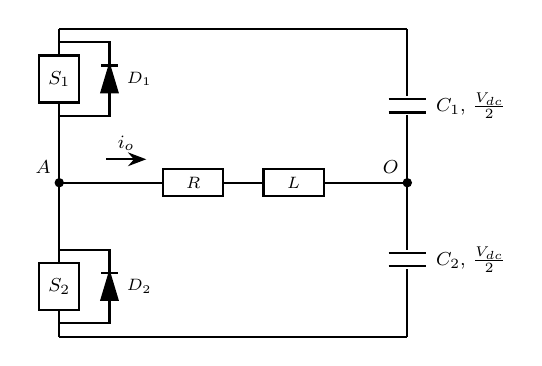
\begin{tikzpicture}[thick,scale=0.85,transform shape]
 \draw (0,2.3)--(5.2,2.3) (0,-2.3)--(5.2,-2.3);
 \swleg{0}{1.55}{$S_1$}{$D_1$} \swleg{0}{-1.55}{$S_2$}{$D_2$}
 \draw (0,0.8)--(0,-0.8) (5.2,2.3)--(5.2,-2.3);
 \capplate{5.2}{1.15} \capplate{5.2}{-1.15}
 \node[font=\footnotesize,right] at (5.5,1.15) {$C_1$, $\tfrac{V_{dc}}{2}$}; \node[font=\footnotesize,right] at (5.5,-1.15) {$C_2$, $\tfrac{V_{dc}}{2}$};
 \draw (0,0)--(5.2,0); \zbox{2.0}{0}{0.9}{$R$} \zbox{3.5}{0}{0.9}{$L$}
 \fill (0,0) circle (2pt) node[above left,font=\footnotesize]{$A$}; \fill (5.2,0) circle (2pt) node[above left,font=\footnotesize]{$O$};
 \draw[-{Stealth}] (0.7,0.35)--(1.3,0.35) node[midway,above,font=\footnotesize]{$i_o$};
\end{tikzpicture}
\caption{Single-phase half-bridge inverter: two switches with anti-parallel feedback diodes and a split DC supply formed by $C_1=C_2$, each holding $V_{dc}/2$. The load connects the leg mid-point $A$ to the centre tap $O$. (Redrawn; compare Hart Fig.~8-8.)}
\label{fig:half_bridge}
\end{figure}

\begin{itemize}[leftmargin=*]
  \item \textbf{Interval 1 ($0 \le t < T/2$):} Switch $S_1$ is turned ON. Load terminal $A$ is connected to the positive DC rail ($+V_{dc}/2$ relative to center tap $O$):
  \begin{equation}
  v_o(t) = v_{AO}(t) = +\frac{V_{dc}}{2}
  \end{equation}
  \item \textbf{Interval 2 ($T/2 \le t < T$):} Switch $S_1$ is turned OFF, and $S_2$ is turned ON. Load terminal $A$ is connected to the negative DC rail ($-V_{dc}/2$):
  \begin{equation}
  v_o(t) = v_{AO}(t) = -\frac{V_{dc}}{2}
  \end{equation}
  \item \textbf{Freewheeling Diode Operation with Inductive Load:} If $S_1$ turns OFF while positive load current $i_o > 0$ is still flowing, inductor energy forces diode $D_2$ into conduction, clamping $v_o = -V_{dc}/2$ and feeding reactive energy back into the lower DC capacitor $C_2$ until $i_o$ decays to zero!
  \item \textbf{RMS Output Voltage:}
  \begin{equation}
  V_{or} = \sqrt{\frac{1}{T}\left[ \int_0^{T/2} \left(+\frac{V_{dc}}{2}\right)^2 dt + \int_{T/2}^T \left(-\frac{V_{dc}}{2}\right)^2 dt \right]} = \frac{V_{dc}}{2}
  \end{equation}
  \item \textbf{Major Limitations of the Half-Bridge Inverter:}
  \begin{enumerate}
    \item Requires a split three-wire DC supply or large center-tapped balancing capacitors.
    \item DC bus voltage utilization is low: the maximum peak-to-peak output voltage is only $V_{dc}$, yielding a fundamental peak of only $\hat{V}_{o1} = \frac{2}{\pi}V_{dc} \approx 0.637 V_{dc}$.
    \item Peak blocking voltage across the OFF-state switch equals the full DC supply $V_{dc} = 2 \times (V_{dc}/2)$, requiring devices rated for twice the output voltage!
  \end{enumerate}
\end{itemize}

\subsubsection{Single-Phase Full-Bridge (H-Bridge) Inverter Configuration}
The full-bridge inverter (Figure~\ref{fig:full_bridge}) eliminates the center-tap requirement by employing four controlled semiconductor switches ($S_1, S_2, S_3, S_4$) arranged in two phase legs ($A$ and $B$) across a single DC source $V_{dc}$.

\begin{figure}[htbp]
\centering
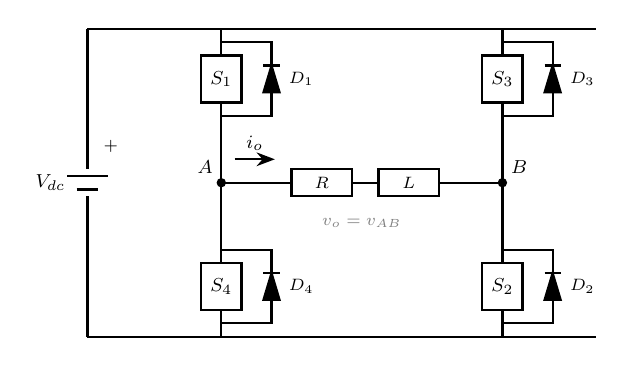
\begin{tikzpicture}[thick,scale=0.85,transform shape]
 \draw (-2,2.3)--(5.6,2.3) (-2,-2.3)--(5.6,-2.3) (-2,2.3)--(-2,-2.3);
 \cellplate{-2}{0} \node[font=\footnotesize,left] at (-2.2,0) {$V_{dc}$}; \node[font=\scriptsize] at (-1.65,0.55) {$+$};
 \swleg{0}{1.55}{$S_1$}{$D_1$} \swleg{0}{-1.55}{$S_4$}{$D_4$}
 \swleg{4.2}{1.55}{$S_3$}{$D_3$} \swleg{4.2}{-1.55}{$S_2$}{$D_2$}
 \draw (0,0.8)--(0,-0.8) (4.2,0.8)--(4.2,-0.8);
 \draw (0,0)--(4.2,0); \zbox{1.5}{0}{0.9}{$R$} \zbox{2.8}{0}{0.9}{$L$}
 \fill (0,0) circle (2pt) node[above left,font=\footnotesize]{$A$}; \fill (4.2,0) circle (2pt) node[above right,font=\footnotesize]{$B$};
 \draw[-{Stealth}] (0.2,0.35)--(0.8,0.35) node[midway,above,font=\footnotesize]{$i_o$};
 \node[font=\scriptsize,gray] at (2.1,-0.6) {$v_o=v_{AB}$};
\end{tikzpicture}
\caption{Single-phase full-bridge (H-bridge) inverter: leg~$A$ ($S_1$, $S_4$) and leg~$B$ ($S_3$, $S_2$), each switch with an anti-parallel diode, across one DC source $V_{dc}$; $v_o=v_{AB}$. (Redrawn; compare Hart Fig.~8-4.)}
\label{fig:full_bridge}
\end{figure}

\begin{itemize}[leftmargin=*]
  \item \textbf{Diagonal Pair Conduction:}
  \begin{itemize}
    \item When switches $(S_1, S_2)$ are gated ON: $v_{Ao} = +V_{dc}/2$ and $v_{Bo} = -V_{dc}/2$, producing output voltage:
    \begin{equation}
    v_o(t) = v_{AB}(t) = v_{Ao} - v_{Bo} = +V_{dc}
    \end{equation}
    \item When switches $(S_3, S_4)$ are gated ON: $v_{Ao} = -V_{dc}/2$ and $v_{Bo} = +V_{dc}/2$, producing output voltage:
    \begin{equation}
    v_o(t) = v_{AB}(t) = -V_{dc}
    \end{equation}
  \end{itemize}
  \item \textbf{RMS Output Voltage:}
  \begin{equation}
  V_{or} = \sqrt{\frac{1}{T}\int_0^T (\pm V_{dc})^2 dt} = V_{dc}
  \end{equation}
  The full-bridge produces \textbf{twice} the output voltage of the half-bridge for the same DC link voltage, yielding four times the output power into a given load resistance!
\end{itemize}

\subsection{Fourier Analysis and Harmonic Spectrum of Square-Wave Inverters}

The square-wave output voltage $v_o(t)$ of a full-bridge inverter alternating between $+V_{dc}$ and $-V_{dc}$ possesses \textbf{odd half-wave symmetry}:
\begin{equation}
v_o(\omega t) = -v_o(\omega t + \pi) \quad \text{and} \quad v_o(-\omega t) = -v_o(\omega t)
\end{equation}
Consequently, all DC offset and all even harmonics are identically zero ($a_0 = 0$, $a_n = 0$, $b_n = 0$ for even $n$). The Fourier series contains only odd sine harmonics:
\begin{equation}
b_n = \frac{2}{\pi} \int_0^\pi V_{dc} \sin(n\omega t) d(\omega t) = \frac{2V_{dc}}{n\pi} \left[-\cos(n\omega t)\right]_0^\pi = \frac{2V_{dc}}{n\pi} \left[1 - (-1)^n\right]
\end{equation}
For odd $n$ ($n = 1, 3, 5, 7, \dots$), $1 - (-1)^n = 2$:
\begin{formulabox}[Fourier Series of Single-Phase Full-Bridge Square-Wave Inverter]
\begin{equation}
v_o(t) = \sum_{n=1,3,5,\dots}^{\infty} \frac{4V_{dc}}{n\pi} \sin(n\omega t) = \frac{4V_{dc}}{\pi} \sin(\omega t) + \frac{4V_{dc}}{3\pi} \sin(3\omega t) + \frac{4V_{dc}}{5\pi} \sin(5\omega t) + \dots
\label{eq:fourier_square_full}
\end{equation}
\end{formulabox}

\subsubsection{Key Harmonic Metrics}
\begin{itemize}[leftmargin=*]
  \item \textbf{Peak Amplitude of Fundamental:} $\hat{V}_{o1} = \frac{4V_{dc}}{\pi} \approx 1.273 V_{dc}$.
  \item \textbf{RMS Value of Fundamental:} $V_{o1(rms)} = \frac{\hat{V}_{o1}}{\sqrt{2}} = \frac{4V_{dc}}{\sqrt{2}\pi} = \frac{2\sqrt{2}}{\pi}V_{dc} \approx 0.9003 V_{dc}$.
  \item \textbf{Harmonic Amplitudes:} The amplitude of the $n$-th harmonic decreases inversely with harmonic order:
  \begin{equation}
  \hat{V}_{on} = \frac{\hat{V}_{o1}}{n} \implies \frac{V_{on}}{V_{o1}} = \frac{1}{n}
  \end{equation}
  Specifically: 3rd harmonic is $33.3\%$ of fundamental, 5th harmonic is $20\%$, 7th harmonic is $14.3\%$.
  \item \textbf{Total Harmonic Distortion (THD) of Voltage:}
  \begin{equation}
  \text{THD}_v = \frac{\sqrt{V_{or}^2 - V_{o1(rms)}^2}}{V_{o1(rms)}} = \frac{\sqrt{V_{dc}^2 - \left(\frac{2\sqrt{2}}{\pi}V_{dc}\right)^2}}{\frac{2\sqrt{2}}{\pi}V_{dc}} = \sqrt{\frac{\pi^2}{8} - 1} \approx \sqrt{1.2337 - 1} = 0.4834 \implies 48.34\%
  \end{equation}
  A total harmonic distortion of $48.34\%$ is severe and unacceptable for sensitive AC loads or utility grid interconnection, motivating the necessity of Pulse Width Modulation (PWM)!
\end{itemize}

\subsection{Square-Wave Inverter with an $RL$ Load: Current Waveform and Conduction Sequence}

With a series $RL$ load, time constant $\tau = L/R$ and period $T = 1/f_o$, the load current is found piece-wise. For $0 \le t < T/2$ the full bridge applies $+V_{dc}$:
\begin{equation}
i_o(t) = \frac{V_{dc}}{R} + \left(I_0 - \frac{V_{dc}}{R}\right)e^{-t/\tau}
\end{equation}
In steady state half-wave symmetry demands $i_o(T/2) = -I_0$, which fixes the starting value:
\begin{formulabox}[Steady-State Load Current of the Square-Wave Inverter ($RL$ load)]
\begin{align}
I_0 &= -\frac{V_{dc}}{R}\,\frac{1 - e^{-T/2\tau}}{1 + e^{-T/2\tau}} = -\frac{V_{dc}}{R}\tanh\!\left(\frac{T}{4\tau}\right), \qquad I_{\max} = -I_0 \notag\\
t_0 &= \tau\ln\!\left[1 + \tanh\!\left(\frac{T}{4\tau}\right)\right]
\label{eq:vsi_rl_current}
\end{align}
\end{formulabox}
$t_0$ is the instant at which the current crosses zero. Between $0$ and $t_0$ the current is still negative although $v_o = +V_{dc}$: it flows through the \textbf{feedback diodes} and returns energy to the DC source. This is why \emph{every} inverter switch needs an anti-parallel diode.

\begin{table}[htbp]
\centering
\small
\caption{Conduction sequence of the full-bridge square-wave inverter with an $RL$ load (half-bridge: same sequence $D_1\!\to\!S_1\!\to\!D_2\!\to\!S_2$ with $\pm V_{dc}/2$).}
\label{tab:conduction_rl}
\begin{tabularx}{\textwidth}{l c c c Y}
\toprule
\textbf{Interval} & \textbf{Gated pair} & $v_o$ & $i_o$ & \textbf{Conducting devices} \\
\midrule
$0 < \omega t < \omega t_0$ & $S_1, S_2$ & $+V_{dc}$ & $<0$ & $D_1, D_2$ (energy fed back to the source) \\
$\omega t_0 < \omega t < \pi$ & $S_1, S_2$ & $+V_{dc}$ & $>0$ & $S_1, S_2$ (source supplies the load) \\
$\pi < \omega t < \pi + \omega t_0$ & $S_3, S_4$ & $-V_{dc}$ & $>0$ & $D_3, D_4$ (energy fed back) \\
$\pi + \omega t_0 < \omega t < 2\pi$ & $S_3, S_4$ & $-V_{dc}$ & $<0$ & $S_3, S_4$ \\
\bottomrule
\end{tabularx}
\end{table}

\begin{figure}[htbp]
\centering
\includegraphics[width=0.78\textwidth]{fig_fullbridge_waveforms.pdf}
\caption{Full-bridge square-wave inverter, $V_{dc}=48$~V, $R=5\,\Omega$, $L=20$~mH, $50$~Hz (the data of Problem~3): (a) output voltage; (b) exact load current with the devices that carry it, and its fundamental component.}
\label{fig:fullbridge_waveforms}
\end{figure}

By superposition, each voltage harmonic of Eq.~\eqref{eq:fourier_square_full} drives a current harmonic through the load impedance at that frequency:
\begin{equation}
i_o(t) = \sum_{n=1,3,5,\dots}\frac{4V_{dc}}{n\pi Z_n}\sin(n\omega t - \phi_n),\qquad Z_n = \sqrt{R^2 + (n\omega L)^2},\quad \phi_n = \arctan\frac{n\omega L}{R}
\end{equation}
Since $Z_n$ grows with $n$, current harmonics fall off faster than $1/n$ and the current is far smoother than the voltage: the load inductance is a low-pass filter. Real power is delivered only by like-order voltage and current harmonics, $P = \sum_n I_{n(rms)}^2 R$.

\subsection{Single-Pulse-Width Modulation}

In \textbf{single-pulse modulation} there is only \textbf{one pulse per half-cycle}, centred on the middle of the half-cycle, and the output voltage is controlled by the pulse width $\delta$ ($0 \le \delta \le \pi$). For the full bridge, $v_o = +V_{dc}$ for $\frac{\pi-\delta}{2} < \omega t < \frac{\pi+\delta}{2}$, $v_o = -V_{dc}$ in the corresponding interval of the negative half-cycle and $v_o = 0$ elsewhere (the zero state is obtained by turning on $S_1, S_3$ or $S_4, S_2$, which short-circuits the load).
\begin{formulabox}[Single-Pulse PWM of the Full-Bridge Inverter]
\begin{align}
V_{or} &= \sqrt{\frac{2}{2\pi}\int_{(\pi-\delta)/2}^{(\pi+\delta)/2} V_{dc}^2\,d(\omega t)} = V_{dc}\sqrt{\frac{\delta}{\pi}} \\
v_o(t) &= \sum_{n=1,3,5,\dots}\frac{4V_{dc}}{n\pi}\,\sin\!\left(\frac{n\pi}{2}\right)\sin\!\left(\frac{n\delta}{2}\right)\sin(n\omega t)
\label{eq:single_pulse}
\end{align}
\end{formulabox}
The fundamental peak is $\hat V_{o1} = \frac{4V_{dc}}{\pi}\sin\frac{\delta}{2}$ (square wave at $\delta = \pi$). The $n$-th harmonic is eliminated when $\sin\frac{n\delta}{2} = 0$, i.e.\ $\delta = \frac{2\pi}{n}$: $\delta = 120^\circ$ removes the 3rd harmonic and $\delta = 72^\circ$ the 5th. \textbf{Disadvantage:} only one harmonic can be eliminated at a time, and the fundamental falls when $\delta$ is reduced (at $\delta = 120^\circ$ it is $0.866$ of the square-wave value). This motivates multiple-pulse (sinusoidal) PWM, which pushes all low-order harmonics up to the carrier frequency.

\subsection{Sinusoidal Pulse Width Modulation (SPWM)}

In \textbf{Sinusoidal Pulse Width Modulation (SPWM)}, the inverter switches are turned ON and OFF multiple times per half-cycle at a high switching frequency. The widths of the gating pulses are modulated proportionally to the instantaneous amplitude of a sinusoidal reference wave.

\subsubsection{Fundamental Definitions and Modulation Parameters}
\begin{enumerate}[leftmargin=*]
  \item \textbf{Modulating / Reference Wave ($v_{\text{control}}$ or $v_{\text{sine}}$):} A low-frequency sinusoidal voltage whose frequency $f_o$ defines the fundamental output frequency of the inverter, and whose peak amplitude $\hat{V}_{\text{control}}$ dictates the output voltage magnitude.
  \item \textbf{Carrier Wave ($v_{\text{tri}}$):} A high-frequency symmetrical triangular waveform of frequency $f_s$ (or $f_c$) and peak amplitude $\hat{V}_{\text{tri}}$.
  \item \textbf{Amplitude Modulation Index ($m_a$):}
  \begin{formulabox}[Amplitude Modulation Index]
  \begin{equation}
  m_a = \frac{\hat{V}_{\text{control}}}{\hat{V}_{\text{tri}}}
  \label{eq:ma_def}
  \end{equation}
  \end{formulabox}
  $m_a$ governs the amplitude of the fundamental output voltage component.
  \item \textbf{Frequency Modulation Ratio ($m_f$):}
  \begin{formulabox}[Frequency Modulation Ratio]
  \begin{equation}
  m_f = \frac{f_s}{f_o} = \frac{f_{\text{carrier}}}{f_{\text{reference}}}
  \label{eq:mf_def}
  \end{equation}
  \end{formulabox}
  $m_f$ determines the frequency at which switching harmonics appear in the output spectrum.
\end{enumerate}

\subsection{PWM with Bipolar Voltage Switching}

In bipolar voltage switching, the diagonally opposite switch pairs $(S_1, S_2)$ and $(S_3, S_4)$ in the full bridge are switched simultaneously in complementary fashion:
\begin{itemize}[leftmargin=*]
  \item When $v_{\text{control}} > v_{\text{tri}}$: Switches $S_1$ and $S_2$ are ON $\implies v_o(t) = +V_{dc}$.
  \item When $v_{\text{control}} < v_{\text{tri}}$: Switches $S_3$ and $S_4$ are ON $\implies v_o(t) = -V_{dc}$.
\end{itemize}
Because the output voltage transitions directly between the two extreme polarities ($+V_{dc}$ and $-V_{dc}$), this scheme is termed \textbf{bipolar switching}.

\begin{figure}[htbp]
\centering
\includegraphics[width=0.78\textwidth]{fig_spwm_bipolar.pdf}
\caption{Bipolar PWM, $m_a=0.8$, $m_f=15$ (computed): (a) reference and triangular carrier; (b) output $v_o/V_{dc}$ switching between $+1$ and $-1$, dashed: fundamental of amplitude $m_aV_{dc}$; (c) harmonic spectrum (FFT of the simulated waveform) with clusters around $m_f$, $2m_f$, $3m_f$. Compare Mohan Fig.~8-5 (one leg).}
\label{fig:bipolar_pwm}
\end{figure}

\subsubsection{Harmonic Characteristics of Bipolar PWM}
\begin{itemize}[leftmargin=*]
  \item \textbf{Fundamental Peak Voltage in Linear Range ($m_a \le 1.0$):}
  \begin{equation}
  \hat{V}_{o1} = m_a V_{dc} \implies V_{o1(rms)} = \frac{m_a V_{dc}}{\sqrt{2}} \approx 0.707 m_a V_{dc}
  \end{equation}
  The fundamental output voltage is strictly linearly proportional to the modulation index $m_a$.
  \item \textbf{Harmonic Sidebands:} Harmonics appear as sidebands clustered around the carrier frequency and its integer multiples:
  \begin{equation}
  f_h = \left(j \cdot m_f \pm k\right) f_o
  \end{equation}
  where the harmonic order is $h = j \cdot m_f \pm k$. For odd $m_f$, $k$ is \emph{even} when $j$ is odd ($m_f,\ m_f\!\pm\!2,\ 3m_f\!\pm\!2,\dots$) and \emph{odd} when $j$ is even ($2m_f\!\pm\!1,\ 2m_f\!\pm\!3,\dots$), so all even harmonics cancel.
  \item \textbf{Selection Rules for $m_f$:}
  \begin{itemize}
    \item $m_f$ should be chosen as an \textbf{odd integer}. This establishes \textbf{odd half-wave symmetry} ($v_o(\omega t + \pi) = -v_o(\omega t)$), which completely eliminates all even harmonics from the output spectrum!
    \item If $m_f$ is an odd integer, the dominant harmonics occur at $m_f$ and $m_f \pm 2$.
    \item Synchronous PWM ($m_f = \text{integer}$) is essential for $m_f < 21$ to prevent sub-harmonic frequencies. For $m_f > 21$, asynchronous PWM can be utilized.
  \end{itemize}
\end{itemize}

\begin{table}[htbp]
\centering
\small
\caption{Generalised harmonics of bipolar PWM for large odd $m_f$: $\hat V_{oh}/V_{dc}$ for the full bridge (identical to $\hat V_{Ao,h}/(V_{dc}/2)$ of one leg). Values reproduce Mohan Table~8-1 and were re-checked by FFT simulation; entries below $0.01$ are omitted. RMS value of a harmonic $=$ tabulated value $\times V_{dc}/\sqrt{2}$.}
\label{tab:mohan81}
\begin{tabularx}{0.86\textwidth}{l Y Y Y Y Y}
\toprule
$h$ \textbackslash\ $m_a$ & $0.2$ & $0.4$ & $0.6$ & $0.8$ & $1.0$ \\
\midrule
$1$ (fundamental) & $0.2$ & $0.4$ & $0.6$ & $0.8$ & $1.0$ \\
$m_f$ & $1.242$ & $1.15$ & $1.006$ & $0.818$ & $0.601$ \\
$m_f \pm 2$ & $0.016$ & $0.061$ & $0.131$ & $0.220$ & $0.318$ \\
$2m_f \pm 1$ & $0.190$ & $0.326$ & $0.370$ & $0.314$ & $0.181$ \\
$2m_f \pm 3$ & --- & $0.024$ & $0.071$ & $0.139$ & $0.212$ \\
$2m_f \pm 5$ & --- & --- & --- & $0.013$ & $0.033$ \\
$3m_f$ & $0.335$ & $0.123$ & $0.083$ & $0.171$ & $0.113$ \\
$3m_f \pm 2$ & $0.044$ & $0.139$ & $0.203$ & $0.176$ & $0.062$ \\
$3m_f \pm 4$ & --- & $0.012$ & $0.047$ & $0.104$ & $0.157$ \\
\bottomrule
\end{tabularx}
\end{table}

\subsection{PWM with Unipolar Voltage Switching}

In unipolar voltage switching, the two inverter legs are controlled independently by comparing the carrier wave $v_{\text{tri}}$ with two reference sine waves that are $180^\circ$ out of phase:
\begin{itemize}[leftmargin=*]
  \item \textbf{Leg A Control:} $v_{\text{control}}$ is compared with $v_{\text{tri}}$:
  \begin{itemize}
    \item If $v_{\text{control}} > v_{\text{tri}}$: Switch $S_1$ is ON ($v_{Ao} = +V_{dc}/2$).
    \item If $v_{\text{control}} < v_{\text{tri}}$: Switch $S_4$ is ON ($v_{Ao} = -V_{dc}/2$).
  \end{itemize}
  \item \textbf{Leg B Control:} $-v_{\text{control}}$ is compared with $v_{\text{tri}}$:
  \begin{itemize}
    \item If $-v_{\text{control}} > v_{\text{tri}}$: Switch $S_3$ is ON ($v_{Bo} = +V_{dc}/2$).
    \item If $-v_{\text{control}} < v_{\text{tri}}$: Switch $S_2$ is ON ($v_{Bo} = -V_{dc}/2$).
  \end{itemize}
\end{itemize}

\begin{figure}[htbp]
\centering
\includegraphics[width=0.78\textwidth]{fig_spwm_unipolar.pdf}
\caption{Unipolar PWM, $m_a=0.8$, $m_f=14$ (computed): (a) the two references $\pm v_{control}$ against one carrier; (b) three-level output $v_o/V_{dc}$ ($+1$, $0$, $-1$); (c) spectrum: nothing at $m_f$ (marked), first cluster at $2m_f$. The $2m_f\pm1$, $2m_f\pm3$ amplitudes equal the corresponding entries of Table~\ref{tab:mohan81}. Compare Mohan Fig.~8-15.}
\label{fig:unipolar_pwm}
\end{figure}

\subsubsection{The Remarkable Advantages of Unipolar PWM}
During each switching event, the output voltage transitions between \textbf{three voltage levels}: $+V_{dc}$, $0$, and $-V_{dc}$:
\begin{itemize}
  \item During the positive half-cycle of $v_{\text{control}}$, $v_o(t)$ switches between $0$ and $+V_{dc}$.
  \item During the negative half-cycle of $v_{\text{control}}$, $v_o(t)$ switches between $0$ and $-V_{dc}$.
\end{itemize}
\begin{conceptbox}[Why Unipolar Switching Outperforms Bipolar Switching]
\begin{enumerate}
  \item \textbf{Doubling of Effective Switching Frequency:} The output voltage pulses appear at \textbf{twice the carrier frequency} ($2f_s$). The fundamental output voltage equation remains identical:
  \begin{equation}
  \hat{V}_{o1} = m_a V_{dc} \quad (0 \le m_a \le 1.0)
  \end{equation}
  \item \textbf{Cancellation of Harmonics at $m_f$:} Harmonics centered around $m_f, 3m_f, 5m_f, \dots$ are completely cancelled out! The lowest-order harmonic sidebands appear centered around $2m_f$:
  \begin{equation}
  h = 2m_f \pm 1, \quad 2m_f \pm 3
  \end{equation}
  \item \textbf{Dramatically Smaller Output Filter:} Because the lowest harmonic frequency is doubled ($2f_s$), the required inductance and capacitance of the output low-pass filter can each be roughly halved (the $LC$ product falls to about one quarter), slashing converter weight, volume, and cost!
  \item \textbf{Reduced Current Ripple:} Load current ripple is substantially smaller compared to bipolar PWM for identical device switching frequencies.
\end{enumerate}
\end{conceptbox}

\begin{table}[htbp]
\centering
\small
\caption{Comprehensive Comparison: Bipolar vs. Unipolar PWM Schemes}
\label{tab:bipolar_vs_unipolar}
\begin{tabularx}{\textwidth}{l X X}
\toprule
\textbf{Feature} & \textbf{Bipolar PWM} & \textbf{Unipolar PWM} \\
\midrule
\textbf{Output Voltage Levels} & 2 levels: $+V_{dc}, -V_{dc}$ & 3 levels: $+V_{dc}, 0, -V_{dc}$ \\
\textbf{Leg Control} & Legs A and B switched simultaneously & Legs A and B switched independently \\
\textbf{Carrier References} & Single sine wave $v_{\text{control}}$ & Complementary pair: $+v_{\text{control}}, -v_{\text{control}}$ \\
\textbf{Selection of $m_f$} & $m_f$ must be an odd integer & $m_f$ is typically chosen as an even integer \\
\textbf{Effective Output Frequency} & $f_s$ (Carrier frequency) & $2f_s$ (Double carrier frequency) \\
\textbf{Dominant Harmonics} & Clustered around $m_f, 2m_f, 3m_f$ & Absent at $m_f$; first appear around $2m_f$ \\
\textbf{Output Filter Size} & Large & Significantly smaller ($L$ and $C$ each $\approx$ halved, $LC$ product $\approx$ one quarter) \\
\textbf{Switching Stress ($dv/dt$)} & Steps of $2V_{dc}$ across load terminals & Steps of $V_{dc}$ across load terminals \\
\textbf{Control Complexity} & Minimal & Moderately higher \\
\bottomrule
\end{tabularx}
\end{table}

\subsection{Operating Modes: Linear Modulation, Overmodulation, and Square-Wave}

The relationship between the fundamental output voltage $\hat{V}_{o1}$ and the modulation index $m_a$ spans three distinct operational regimes:

\begin{enumerate}[leftmargin=*]
  \item \textbf{Linear Modulation Region ($0 \le m_a \le 1.0$):}
  \begin{itemize}
    \item The peak of the modulating sine wave is less than or equal to the triangular carrier peak ($\hat{V}_{\text{control}} \le \hat{V}_{\text{tri}}$).
    \item The fundamental peak output voltage varies strictly linearly with $m_a$:
    \begin{equation}
    \hat{V}_{o1} = m_a V_{dc}
    \end{equation}
    \item The harmonic frequencies are independent of $m_a$, and harmonic amplitudes are directly proportional to $m_a$.
  \end{itemize}

  \item \textbf{Overmodulation Region ($m_a > 1.0$):}
  \begin{itemize}
    \item The reference amplitude exceeds the carrier peak. Around the sine-wave peaks the reference stays above the carrier for several carrier cycles, so \textbf{pulses are dropped}: the switch stays ON (or OFF) without pulsing.
    \item $\hat{V}_{o1}$ is no longer proportional to $m_a$: it rises ever more slowly from $V_{dc}$ at $m_a = 1$ towards $\frac{4V_{dc}}{\pi}$ (Fig.~\ref{fig:overmod_curve}). In Mohan's one-leg notation, $\frac{V_{dc}}{2} < \hat{V}_{Ao1} < \frac{4}{\pi}\frac{V_{dc}}{2}$.
    \item Low-order harmonics (3rd, 5th, 7th, \dots) reappear and the spectrum becomes sensitive to $m_f$ (Mohan Fig.~8-7), so synchronous PWM is recommended. Overmodulation is avoided in UPS systems (strict distortion limits) but normally used in induction-motor drives to extract more voltage.
  \end{itemize}

  \item \textbf{Square-Wave Operation ($m_a$ very large):}
  \begin{itemize}
    \item The pulses merge into one pulse per half-cycle. The limit $\frac{4V_{dc}}{\pi}$ is approached asymptotically: our simulation ($m_f = 39$) already reaches $98\%$ of it at $m_a \approx 3.2$, which is why books quote a practical threshold of ``$m_a \gtrsim 3$--$4$'' rather than a sharp value.
    \item The fundamental saturates at
    \begin{equation}
    \hat{V}_{o1,\text{max}} = \frac{4V_{dc}}{\pi} \approx 1.273 V_{dc}
    \end{equation}
    i.e.\ $27\%$ more than the linear-range limit $V_{dc}$. Each switch conducts $180^\circ$ and there is no harmonic reduction ($\text{THD}_v = 48.3\%$).
    \item The output is independent of $m_a$ and can only be changed through the DC link voltage $V_{dc}$.
  \end{itemize}
\end{enumerate}

\begin{figure}[htbp]
\centering
\includegraphics[width=0.72\textwidth]{fig_overmod_curve.pdf}
\caption{Fundamental amplitude of the bipolar full-bridge output versus $m_a$ (computed, $m_f = 39$): linear region, over-modulation and approach to the square-wave limit $4/\pi$. Compare Mohan Fig.~8-8.}
\label{fig:overmod_curve}
\end{figure}

\subsection{The Critical Need for Blanking Time (Dead-Time)}

In practical bridge inverters, power semiconductor switches (IGBTs, MOSFETs) do not turn OFF instantaneously due to stored minority carrier recombination and gate charge discharging times ($t_{off} > t_{on}$).

\begin{figure}[htbp]
\centering
\includegraphics[width=0.8\textwidth]{fig_deadtime.pdf}
\caption{Effect of the blanking time $t_d$ on one inverter leg (computed): (a) ideal complementary gate commands; (b) actual gates, both switches OFF for $t_d$ at every transition; (c) pole voltage for $i_o > 0$: the pulse is shortened by $t_d$; (d) pole voltage for $i_o < 0$: the pulse is lengthened by $t_d$. Compare Mohan Fig.~8-31.}
\label{fig:blanking_time}
\end{figure}

\subsubsection{The Shoot-Through Catastrophe}
If the turn-ON command is given to the upper switch ($S_1$) at the same instant as the turn-OFF command to the lower switch ($S_4$) of the same leg, both devices conduct together while the outgoing device is still turning off (turn-off is slower than turn-on, $t_{off} > t_{on}$). This \textbf{shoot-through} is a near short circuit across the DC bus, limited only by parasitic resistance and device drops:
\begin{equation}
I_{\text{fault}} \approx \frac{V_{dc}}{R_{\text{parasitic}}} \to \text{thousands of amperes} \implies \text{device and DC-link destruction}
\end{equation}

\subsubsection{Implementation of Blanking Time ($t_d$ or $t_\Delta$)}
To prevent shoot-through a deliberate delay, the \textbf{blanking time} (dead time) $t_d$, is inserted between the turn-OFF command of one switch and the turn-ON command of the complementary switch of the same leg. The incoming device must not start conducting before the outgoing one has fully turned off:
\begin{equation}
t_d \;>\; t_{off,\max} - t_{d(on),\min} + \Delta t_{\text{driver}}
\end{equation}
where $t_{d(on),\min}$ is the minimum turn-on delay of the incoming device and $\Delta t_{\text{driver}}$ the spread of gate-driver propagation delays. Typical values: $1$--$3\,\mu\text{s}$ for IGBTs; $100$--$500\text{ ns}$ for silicon MOSFETs; $<50\text{ ns}$ for GaN HEMTs.

\subsubsection{Adverse Effects and Voltage Error Caused by Blanking Time}
During $t_d$ both controlled switches of the leg are OFF and the pole voltage is fixed entirely by the \textbf{direction of the load current} through the feedback diodes (Fig.~\ref{fig:blanking_time}):
\begin{itemize}[leftmargin=*]
  \item \textbf{When $i_o > 0$:} the current flows through the lower diode $D_4$, so the pole voltage is $0$ during the dead time even though $S_1$ is commanded ON. The positive pulse is \textbf{shorter by $t_d$}: area $V_{dc}t_d$ is lost.
  \item \textbf{When $i_o < 0$:} the current flows through the upper diode $D_1$ and the pole voltage is $+V_{dc}$ during the dead time. The positive pulse is \textbf{longer by $t_d$}.
  \item The error depends only on the \emph{sign} of the current, not on its magnitude. Averaged over one switching period $T_s$ the pole-voltage error is (Mohan Eq.~8-75):
\end{itemize}
\begin{formulabox}[Average Pole-Voltage Error Due to Blanking Time]
\begin{equation}
\Delta V_{Ao} = \frac{t_d}{T_s}V_{dc}\,\operatorname{sgn}(i_A) = f_s\,t_d\,V_{dc}\,\operatorname{sgn}(i_A) \qquad (\text{a drop when } i_A > 0)
\label{eq:deadtime_voltage_drop}
\end{equation}
\end{formulabox}
In the single-phase full bridge with bipolar switching, leg~$B$ carries $-i_o$ and its error has the opposite sign in $v_{Bo}$, so the two legs add: $\Delta V_o = 2 f_s t_d V_{dc}\operatorname{sgn}(i_o)$ (Mohan Eq.~8-77). The error is therefore a \textbf{square wave in phase with the load current}: its amplitude is $f_s t_d V_{dc}$ per leg and its fundamental component has peak $\frac{4}{\pi}f_s t_d V_{dc}$ (the factor $\frac{4}{\pi}$ comes from the Fourier series of the square wave, not from the averaging).
\begin{itemize}[leftmargin=*]
  \item \textbf{Consequences:}
  \begin{enumerate}
    \item The fundamental output voltage is reduced, most noticeably at low modulation index (the error is a fixed voltage, independent of $m_a$).
    \item Low-order harmonics appear: 3rd, 5th, 7th in a single-phase inverter; 5th, 7th, 11th, 13th in a three-phase inverter. They cause torque pulsation in AC motors.
    \item The output voltage is distorted around the current zero crossings.
  \end{enumerate}
  \item \textbf{Remedy:} dead-time compensation, i.e.\ detect the sign of the phase current and add $\pm f_s t_d V_{dc}$ to the voltage command, and use fast devices so that a small $t_d$ is sufficient.
\end{itemize}


\section{Three-Phase Pulse Width Modulated Voltage Source Inverters}

\subsection{Three-Phase Bridge Inverter Topology and Conduction Mechanics}

The three-phase voltage source inverter (Figure~\ref{fig:3ph_inverter_ckt}) is the universal industry-standard power conversion topology for variable-frequency AC motor drives (VFDs), grid-tied solar photovoltaic central inverters, wind turbine grid converters, and electric vehicle traction drives ($50\text{ kW} - 300\text{ kW}$).

The topology comprises six controlled switches ($S_1$ through $S_6$) arranged in three inverter legs ($A, B, C$) across a common DC link voltage $V_{dc}$, with six anti-parallel freewheeling diodes ($D_1$ through $D_6$).

\begin{figure}[htbp]
\centering
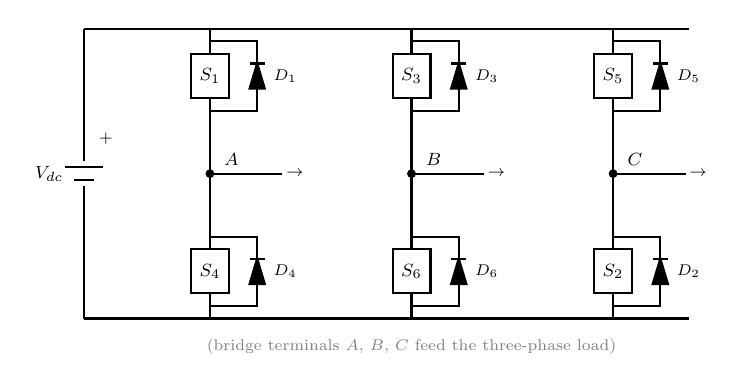
\begin{tikzpicture}[thick,scale=0.8,transform shape]
 \draw (-2,2.3)--(7.6,2.3) (-2,-2.3)--(7.6,-2.3) (-2,2.3)--(-2,-2.3);
 \cellplate{-2}{0} \node[font=\footnotesize,left] at (-2.2,0) {$V_{dc}$}; \node[font=\scriptsize] at (-1.65,0.55) {$+$};
 \swleg{0}{1.55}{$S_1$}{$D_1$} \swleg{0}{-1.55}{$S_4$}{$D_4$}
 \swleg{3.2}{1.55}{$S_3$}{$D_3$} \swleg{3.2}{-1.55}{$S_6$}{$D_6$}
 \swleg{6.4}{1.55}{$S_5$}{$D_5$} \swleg{6.4}{-1.55}{$S_2$}{$D_2$}
 \draw (0,0.8)--(0,-0.8) (3.2,0.8)--(3.2,-0.8) (6.4,0.8)--(6.4,-0.8);
 \foreach \x/\n in {0/A,3.2/B,6.4/C}{ \fill (\x,0) circle (2pt); \draw (\x,0)--(\x+1.15,0); \node[font=\footnotesize,above right] at (\x+0.1,0) {$\n$}; \node[font=\scriptsize] at (\x+1.35,0) {$\to$};}
 \node[font=\scriptsize,gray] at (3.2,-2.75) {(bridge terminals $A$, $B$, $C$ feed the three-phase load)};
\end{tikzpicture}
\caption{Three-phase voltage source inverter: three legs $A$, $B$, $C$ (upper switches $S_1, S_3, S_5$; lower switches $S_4, S_6, S_2$), each with an anti-parallel diode, across the DC link $V_{dc}$. The load may be star or delta connected. (Redrawn; compare Mohan Fig.~8-21.)}
\label{fig:3ph_inverter_ckt}
\end{figure}

\subsubsection{Switch Numbering and Firing Sequence}
The switches are traditionally numbered according to their natural firing sequence in a balanced three-phase cycle:
\begin{itemize}[leftmargin=*]
  \item Upper switches: $S_1$ (Phase A), $S_3$ (Phase B), $S_5$ (Phase C).
  \item Lower switches: $S_4$ (Phase A), $S_6$ (Phase B), $S_2$ (Phase C).
  \item Firing sequence: $S_1 \to S_2 \to S_3 \to S_4 \to S_5 \to S_6$, spaced by intervals of $60^\circ$ ($\pi/3$).
\end{itemize}

\subsection{Sinusoidal PWM in Three-Phase VSIs}

In three-phase SPWM, three balanced sinusoidal reference voltages displaced by $120^\circ$ are compared against a common high-frequency triangular carrier wave $v_{\text{tri}}$:
\begin{align}
v_{\text{control},A} &= \hat{V}_{\text{control}} \sin(\omega t) \notag\\
v_{\text{control},B} &= \hat{V}_{\text{control}} \sin(\omega t - 120^\circ) \notag\\
v_{\text{control},C} &= \hat{V}_{\text{control}} \sin(\omega t - 240^\circ) = \hat{V}_{\text{control}} \sin(\omega t + 120^\circ)
\end{align}

\begin{figure}[htbp]
\centering
\includegraphics[width=0.78\textwidth]{fig_3ph_spwm.pdf}
\caption{Three-phase SPWM, $m_a=0.8$, $m_f=15$ (computed): (a) three references $120^\circ$ apart and one carrier; (b) pole voltage $v_{Ao}/V_{dc}$ (two levels, fundamental $m_a/2$); (c) line voltage $v_{AB}/V_{dc} = v_{Ao}-v_{Bo}$ (levels $+1, 0, -1$, fundamental $0.866\,m_a$); (d) spectrum of $v_{AB}$: the $h=m_f=15$ component and all triplen harmonics are absent. Compare Mohan Fig.~8-22.}
\label{fig:3ph_pwm_waveforms}
\end{figure}

\subsubsection{Pole Voltages and Line-to-Line Voltages}
Each leg operates identically to a single-phase half-bridge pole relative to the fictitious DC-bus midpoint $o$:
\begin{equation}
v_{Ao}(t) = \begin{cases} +V_{dc}/2, & \text{if } v_{\text{control},A} > v_{\text{tri}} \\ -V_{dc}/2, & \text{if } v_{\text{control},A} < v_{\text{tri}} \end{cases}
\end{equation}
The line-to-line output voltages are obtained by taking the difference between individual leg pole voltages:
\begin{align}
v_{AB}(t) &= v_{Ao}(t) - v_{Bo}(t) \notag\\
v_{BC}(t) &= v_{Bo}(t) - v_{Co}(t) \notag\\
v_{CA}(t) &= v_{Co}(t) - v_{Ao}(t)
\end{align}

\subsubsection{Cancellation of Triplen Harmonics in Three-Phase PWM}
A fundamental property of three-phase balanced systems is that \textbf{all triplen harmonics ($n = 3, 9, 15, 21, \dots$) are identical in magnitude and in-phase across all three phase legs}:
\begin{equation}
v_{Ao,3}(t) = v_{Bo,3}(t) = v_{Co,3}(t)
\end{equation}
Taking the line-to-line difference completely cancels all triplen harmonics:
\begin{equation}
v_{AB,3}(t) = v_{Ao,3}(t) - v_{Bo,3}(t) \equiv 0!
\end{equation}
\begin{conceptbox}[Fundamental Voltage Relationships in 3-Phase SPWM]
In the linear modulation range ($0 \le m_a \le 1.0$):
\begin{enumerate}
  \item \textbf{Peak Fundamental Pole-to-Midpoint Voltage:}
  \begin{equation}
  \hat{V}_{Ao1} = m_a \frac{V_{dc}}{2}
  \end{equation}
  \item \textbf{Peak Fundamental Line-to-Line Voltage:}
  \begin{equation}
  \hat{V}_{LL1} = \sqrt{3} \hat{V}_{Ao1} = \sqrt{3} m_a \frac{V_{dc}}{2} = \frac{\sqrt{3}}{2} m_a V_{dc} \approx 0.866 m_a V_{dc}
  \label{eq:vll1_peak}
  \end{equation}
  \item \textbf{RMS Fundamental Line-to-Line Voltage:}
  \begin{equation}
  V_{LL1(rms)} = \frac{\hat{V}_{LL1}}{\sqrt{2}} = \frac{\sqrt{3}}{2\sqrt{2}} m_a V_{dc} = \frac{\sqrt{6}}{4} m_a V_{dc} \approx 0.6124 m_a V_{dc}
  \label{eq:vll1_rms}
  \end{equation}
  \item \textbf{Maximum Linear Line-to-Line RMS Voltage ($m_a = 1.0$):}
  \begin{equation}
  V_{LL1(rms),\text{max}} = 0.6124 V_{dc}
  \end{equation}
\end{enumerate}
\end{conceptbox}

\subsubsection{Three-Phase Frequency Modulation Ratio ($m_f$) Selection Criteria}
To ensure optimum harmonic elimination in three-phase inverters, $m_f$ must adhere to two strict design criteria:
\begin{enumerate}
  \item $m_f$ must be an \textbf{odd integer}: Ensures half-wave symmetry, completely eliminating all even harmonics.
  \item $m_f$ must be an \textbf{odd multiple of 3} ($m_f = 9, 15, 21, 27, 33, \dots$):
  \begin{itemize}
    \item The strongest carrier harmonic of every leg is the one at $h = m_f$ itself. The legs are displaced by $120^\circ$ at the fundamental, so this harmonic is displaced by $120^\circ \times m_f$, which is a multiple of $360^\circ$ when $m_f$ is a multiple of 3: it is then \textbf{identical in all three pole voltages}.
    \item Hence the $m_f$ harmonic (and its odd multiples $3m_f, 5m_f, \dots$) is \textbf{cancelled in the line-to-line voltage}.
    \item The lowest carrier-related harmonics left in $v_{AB}$ are the sidebands $(m_f \pm 2)$, followed by the much smaller $(m_f \pm 4)$ (Fig.~\ref{fig:3ph_pwm_waveforms}d).
  \end{itemize}
\end{enumerate}

\subsection{Overmodulation and Square-Wave Operation in Three-Phase Inverters}

\subsubsection{Overmodulation Region ($m_a > 1.0$)}
When $m_a$ exceeds $1.0$ the reference peaks exceed the carrier and pulses are dropped. The fundamental line-to-line voltage keeps rising beyond $0.6124\,V_{dc}$ (RMS) towards the six-step value $0.7797\,V_{dc}$, but no longer in proportion to $m_a$, and low-order non-triplen harmonics (5th, 7th, 11th, 13th) re-appear in $v_{AB}$.

\subsubsection{Square-Wave (Six-Step) Operation}
For very large $m_a$ (practically $m_a \gtrsim 3$--$4$; the limit is reached only asymptotically) the inverter becomes the classical \textbf{six-step (180$^\circ$ conduction) inverter}. Each switch conducts for $180^\circ$, the switching instants are $60^\circ$ apart, and at any instant exactly three switches (one per leg) are ON.

\begin{figure}[htbp]
\centering
\includegraphics[width=0.78\textwidth]{fig_six_step.pdf}
\caption{Six-step operation (computed, $\pm V_{dc}/2$ pole voltages): (a) pole voltages displaced by $120^\circ$; (b) phase voltage $v_{AN}$ of a star load, a six-step staircase with levels $\pm\frac{1}{3}V_{dc}$ and $\pm\frac{2}{3}V_{dc}$; (c) line voltage $v_{AB}$, $120^\circ$ wide pulses separated by $60^\circ$ zero intervals.}
\label{fig:six_step}
\end{figure}

\begin{table}[htbp]
\centering
\small
\caption{Six-step ($180^\circ$ conduction) inverter, star load: conducting switches and voltages in units of $V_{dc}$ (time origin: $S_1$ turned on at $\omega t = 0$).}
\label{tab:six_step_modes}
\begin{tabularx}{\textwidth}{c c c c c c}
\toprule
\textbf{Interval} & \textbf{Switches ON} & $v_{AN}$ & $v_{BN}$ & $v_{CN}$ & $v_{AB}$ \\
\midrule
$0^\circ$--$60^\circ$ & $S_5, S_6, S_1$ & $+\frac{1}{3}$ & $-\frac{2}{3}$ & $+\frac{1}{3}$ & $+1$ \\
$60^\circ$--$120^\circ$ & $S_6, S_1, S_2$ & $+\frac{2}{3}$ & $-\frac{1}{3}$ & $-\frac{1}{3}$ & $+1$ \\
$120^\circ$--$180^\circ$ & $S_1, S_2, S_3$ & $+\frac{1}{3}$ & $+\frac{1}{3}$ & $-\frac{2}{3}$ & $0$ \\
$180^\circ$--$240^\circ$ & $S_2, S_3, S_4$ & $-\frac{1}{3}$ & $+\frac{2}{3}$ & $-\frac{1}{3}$ & $-1$ \\
$240^\circ$--$300^\circ$ & $S_3, S_4, S_5$ & $-\frac{2}{3}$ & $+\frac{1}{3}$ & $+\frac{1}{3}$ & $-1$ \\
$300^\circ$--$360^\circ$ & $S_4, S_5, S_6$ & $-\frac{1}{3}$ & $-\frac{1}{3}$ & $+\frac{2}{3}$ & $0$ \\
\bottomrule
\end{tabularx}
\end{table}

\begin{itemize}[leftmargin=*]
  \item Two legs on the same side connect two load phases in parallel, which then sit in series with the third phase: this is where the levels $\frac{1}{3}$ and $\frac{2}{3}$ come from.
  \item The line-to-line voltage is a six-step waveform alternating between $+V_{dc}$, $0$ and $-V_{dc}$. With the time origin at the centre of the positive pulse of $v_{AB}$, its Fourier series is:
  \begin{equation}
  v_{AB}(t) = \sum_{n=1,5,7,11,13,\dots}^{\infty} \frac{4V_{dc}}{n\pi} \cos\left(\frac{n\pi}{6}\right) \sin(n\omega t)
  \end{equation}
  For all triplen harmonics ($n = 3, 9, 15, \dots$), $\cos(n\pi/6) = 0$: complete triplen elimination.
  \item \textbf{Peak Fundamental Line-to-Line Voltage:}
  \begin{equation}
  \hat{V}_{LL1,\text{square}} = \frac{4V_{dc}}{\pi} \cos\left(\frac{\pi}{6}\right) = \frac{2\sqrt{3}}{\pi}V_{dc} \approx 1.1027 V_{dc}
  \end{equation}
  \item \textbf{RMS Fundamental Line-to-Line Voltage:}
  \begin{equation}
  V_{LL1(rms),\text{square}} = \frac{\hat{V}_{LL1,\text{square}}}{\sqrt{2}} = \frac{\sqrt{6}}{\pi}V_{dc} \approx 0.7797 V_{dc}
  \end{equation}
  \item \textbf{Total RMS Line-to-Line Voltage:}
  \begin{equation}
  V_{LL(rms)} = \sqrt{\frac{1}{\pi} \int_0^{2\pi/3} V_{dc}^2 d(\omega t)} = V_{dc}\sqrt{\frac{2}{3}} \approx 0.8165 V_{dc}
  \end{equation}
  \item \textbf{Phase (line-to-neutral) voltage of a star load:} the staircase $v_{AN}$ has
  \begin{align}
  v_{AN}(t) &= \sum_{n=1,5,7,11,13,\dots}\frac{2V_{dc}}{n\pi}\sin(n\omega t) \notag\\
  \hat{V}_{AN1} &= \frac{2V_{dc}}{\pi} \approx 0.637V_{dc},\quad V_{AN1(rms)} \approx 0.450V_{dc},\quad V_{AN(rms)} = \frac{\sqrt{2}}{3}V_{dc} \approx 0.471V_{dc} \notag
  \end{align}
  consistent with $V_{LL} = \sqrt{3}\,V_{AN}$ ($0.8165 = \sqrt{3}\times 0.4714$).
  \item \textbf{Distortion:} $\text{THD}_v = \sqrt{(0.8165/0.7797)^2 - 1} \approx 31.1\%$ for both line and phase voltages (compare $48.3\%$ for the single-phase square wave).
\end{itemize}

\subsection{Third Harmonic Injection PWM (THIPWM)}

In standard sinusoidal PWM, the maximum linear fundamental line-to-line voltage is limited to $\hat{V}_{LL1} = \frac{\sqrt{3}}{2}V_{dc} \approx 0.866 V_{dc}$ because the peak of each phase reference sine wave cannot exceed the DC rails ($\pm V_{dc}/2$) without causing overmodulation distortion.

\begin{figure}[htbp]
\centering
\includegraphics[width=0.78\textwidth]{fig_thipwm.pdf}
\caption{Third-harmonic injection PWM (computed): (a) $\sin\omega t + \frac{1}{6}\sin 3\omega t$ peaks at only $0.866$ (at $60^\circ$ and $120^\circ$), with a shallow dip to $0.833$ at $90^\circ$; (b) after boosting the fundamental by $2/\sqrt{3}$ the three references just touch the carrier peak, while $v_A - v_B$ remains a pure sinusoid.}
\label{fig:thipwm}
\end{figure}

\begin{figure}[htbp]
\centering
\includegraphics[width=0.55\textwidth]{mod_p52_img1.jpeg}
\caption{Lecture slide: output versus modulation index $M$. Harmonic injection extends the linear range beyond $M=1$ (green) before over-modulation begins (red). (Source: lecture slides)}
\label{fig:thipwm_slide}
\end{figure}

\subsubsection{Mathematical Formulation of THIPWM}
A zero-sequence third harmonic, identical in all three phases, is added to each sinusoidal reference:
\begin{align}
v_{\text{control},A}(t) &= \hat{V}_1 \left[ \sin(\omega t) + \tfrac{1}{6} \sin(3\omega t) \right] \notag\\
v_{\text{control},B}(t) &= \hat{V}_1 \left[ \sin(\omega t - 120^\circ) + \tfrac{1}{6} \sin(3\omega t) \right] \notag\\
v_{\text{control},C}(t) &= \hat{V}_1 \left[ \sin(\omega t + 120^\circ) + \tfrac{1}{6} \sin(3\omega t) \right]
\label{eq:thipwm_formula}
\end{align}
(the third harmonic of $\sin(\omega t \mp 120^\circ)$ is $\sin(3\omega t \mp 360^\circ) = \sin 3\omega t$ in every phase). The injected amplitude $\frac{1}{6} \approx 16.7\%$ of the fundamental is the value that gives the largest linear range.

\subsubsection{Why Third Harmonic Injection Works}
\begin{conceptbox}[Physics of Third Harmonic Injection]
\begin{enumerate}
  \item \textbf{The peak of the composite reference is lower than the fundamental's.} Setting the derivative of $f(\theta) = \sin\theta + \frac{1}{6}\sin 3\theta$ to zero and using $\cos 3\theta = 4\cos^3\theta - 3\cos\theta$:
  \begin{align}
  f'(\theta) &= \cos\theta + \tfrac{1}{2}\cos 3\theta = \tfrac{1}{2}\cos\theta\,\left(4\cos^2\theta - 1\right) = 0 \notag\\
  &\implies \cos\theta = 0 \ \text{or}\ \cos\theta = \pm\tfrac{1}{2} \notag
  \end{align}
  At $\theta = 60^\circ$ and $120^\circ$ the maxima are $f = \frac{\sqrt{3}}{2} \approx 0.866$; at $\theta = 90^\circ$ there is only a shallow dip, $f = 1 - \frac{1}{6} = \frac{5}{6} \approx 0.833$. So the peak is flattened to $0.866$ of the fundamental amplitude.
  \item \textbf{15.5\% voltage boost in the linear range.} The fundamental can therefore be raised by $\frac{2}{\sqrt{3}} \approx 1.1547$ before the composite reference touches the carrier peak, i.e.\ $m_a$ may go up to $1.1547$ without over-modulation:
  \begin{align}
  \hat{V}_{LL1,\text{max (THIPWM)}} &= \frac{\sqrt{3}}{2}\,(1.1547)\,V_{dc} = 1.000\,V_{dc} \notag\\
  V_{LL1(rms),\text{max (THIPWM)}} &= \frac{V_{dc}}{\sqrt{2}} \approx 0.707\,V_{dc} \notag
  \end{align}
  compared with $0.612\,V_{dc}$ for ordinary SPWM: a gain of $15.5\%$ without leaving the linear region.
  \item \textbf{No distortion at the load.} The injected term is the same in all three phases (zero-sequence), so it cancels in every line-to-line voltage:
  \begin{equation}
  v_{AB}(t) = v_{Ao}(t) - v_{Bo}(t) = \text{pure fundamental (+ switching harmonics)}
  \end{equation}
  and, with an isolated star point, it drives no load current.
  \item \textbf{Same DC-bus utilisation as space-vector PWM.} Space-vector modulation reaches the same maximum linear output ($1.1547$ in $m_a$ terms); it effectively injects a triangular (min--max) zero-sequence signal instead of a sinusoidal third harmonic, but THIPWM achieves the same range with simple carrier comparators.
\end{enumerate}
\end{conceptbox}

\begin{table}[htbp]
\centering
\small
\caption{Maximum fundamental line-to-line RMS voltage of a three-phase inverter, as a fraction of $V_{dc}$.}
\label{tab:max_vll}
\begin{tabularx}{0.8\textwidth}{l Y Y}
\toprule
\textbf{Modulation} & $V_{LL1(rms),\max}/V_{dc}$ & \textbf{Relative to SPWM} \\
\midrule
SPWM, linear range ($m_a = 1$) & $0.612$ & $1.000$ \\
THIPWM / SVPWM, linear range & $0.707$ & $1.155$ \\
Six-step (square wave) & $0.780$ & $1.273$ \\
\bottomrule
\end{tabularx}
\end{table}


\section{Current Source Inverters (CSI) and Detailed Comparison with VSI}

\subsection{Operating Principle of Single-Phase Current Source Inverters (CSI)}

In contrast to a Voltage Source Inverter (which is fed from a stiff, low-impedance DC voltage source), a \textbf{Current Source Inverter (CSI)} is fed from an adjustable direct current source possessing \textbf{high internal impedance}. In practice, this is realized by placing a large smoothing choke ($L_{dc}$) in series with a controlled DC power supply or phase-controlled thyristor rectifier.

\begin{figure}[htbp]
\centering
\begin{circuitikz}[thick,scale=0.9,transform shape]
 % DC current source and smoothing choke
 \draw (0,0) to[isource, l_=$I_{dc}$] (0,3.6);
 \draw (0,3.6)--(0.6,3.6) to[L, l=$L_{dc}$] (2.8,3.6)--(8.4,3.6);
 \draw (0,0)--(8.4,0);
 % left leg: S1, D1 | node A | D4, S4
 \draw (4.2,3.6)--(4.2,3.4); \sbx{4.2}{3.1}{$S_1$}; \draw (4.2,2.8)--(4.2,2.6); \dn{4.2}{2.6}{$D_1$}; \draw (4.2,2.25)--(4.2,1.4);
 \draw (4.2,1.4)--(4.2,1.3); \dn{4.2}{1.3}{$D_4$}; \draw (4.2,0.95)--(4.2,0.8); \sbx{4.2}{0.5}{$S_4$}; \draw (4.2,0.2)--(4.2,0);
 % right leg: S3, D3 | node B | D2, S2
 \draw (7.0,3.6)--(7.0,3.4); \sbx{7.0}{3.1}{$S_3$}; \draw (7.0,2.8)--(7.0,2.6); \dn{7.0}{2.6}{$D_3$}; \draw (7.0,2.25)--(7.0,1.4);
 \draw (7.0,1.4)--(7.0,1.3); \dn{7.0}{1.3}{$D_2$}; \draw (7.0,0.95)--(7.0,0.8); \sbx{7.0}{0.5}{$S_2$}; \draw (7.0,0.2)--(7.0,0);
 % load between A and B
 \fill (4.2,1.8) circle (2pt) node[left,font=\footnotesize]{$A$}; \fill (7.0,1.8) circle (2pt) node[right,font=\footnotesize]{$B$};
 \draw (4.2,1.8)--(5.2,1.8); \draw[thick,fill=white] (5.2,1.55) rectangle (6.0,2.05); \node[font=\footnotesize] at (5.6,1.8) {Load}; \draw (6.0,1.8)--(7.0,1.8);
 \draw[-{Stealth}] (5.0,2.3)--(6.2,2.3) node[midway,above,font=\scriptsize]{$i_o$ for $S_1,S_2$ on};
\end{circuitikz}
\caption{Single-phase IGBT-based Current Source Inverter (CSI) with series blocking diodes and massive DC smoothing inductor $L_{dc}$.}
\label{fig:csi_circuit}
\end{figure}

\subsubsection{Circuit Characteristics of the CSI}
\begin{enumerate}[leftmargin=*]
  \item \textbf{Constant Input Current ($I_{dc}$):} Due to the large inductance $L_{dc}$, the DC link current cannot change instantaneously:
  \begin{equation}
  i_{dc}(t) \approx I_{dc} = \text{constant (ripple-free)}
  \end{equation}
  \item \textbf{Square-Wave Output Current Waveform:} Gating switch pair $(S_1, S_2)$ directs $+I_{dc}$ through the load, while gating $(S_3, S_4)$ directs $-I_{dc}$ through the load. The output current $i_o(t)$ is therefore a \textbf{clean square wave alternating between $+I_{dc}$ and $-I_{dc}$}.
  \item \textbf{Need for Series Blocking Diodes ($D_1 - D_4$):}
  \begin{itemize}
    \item Standard power MOSFETs and IGBTs have anti-parallel body diodes or low reverse-blocking voltage ratings ($< 20\text{ V}$).
    \item In a CSI, the load voltage is alternating AC, meaning the switches must withstand \textbf{large reverse voltages}.
    \item Fast-recovery diodes are placed strictly in \textbf{series} with each controlled switch to provide the necessary reverse voltage blocking capability!
  \end{itemize}
  \item \textbf{Inherent Short-Circuit Immunity:} In a VSI, accidental simultaneous conduction of upper and lower switches causes an explosive shoot-through short circuit. In sharp contrast, in a CSI, \textbf{simultaneous conduction of upper and lower switches merely circulates the constant DC current $I_{dc}$ without any current spike!}
  \item \textbf{Open-Circuit Danger:} In a CSI, an open circuit in the load or DC path is catastrophic ($L \frac{di}{dt} \to \infty$, generating thousands of volts of inductive overvoltage arc breakdown). An overlap period is mandatory during commutation!
\end{enumerate}

\subsubsection{Output Current of the Single-Phase CSI (Dual of the VSI Voltage)}
With ideal switches and a constant $I_{dc}$, the output current is a square wave of amplitude $\pm I_{dc}$, the exact dual of the VSI output voltage:
\begin{align}
i_o(t) &= \sum_{n=1,3,5,\dots}\frac{4I_{dc}}{n\pi}\sin(n\omega t) \notag\\
\hat{I}_{o1} &= \frac{4I_{dc}}{\pi} \approx 1.273I_{dc}, \qquad I_{o1(rms)} = \frac{2\sqrt{2}}{\pi}I_{dc} \approx 0.900I_{dc}, \qquad \text{THD}_i = 48.3\% \notag
\end{align}
The output \emph{voltage} is not imposed by the switches but developed by this current in the load. A parallel $RLC$ load tuned to $f_o$ (high $Q$) offers a high impedance only at the fundamental, so the harmonic currents produce almost no voltage and $v_o$ is nearly sinusoidal (Fig.~\ref{fig:csi_waveforms}).

\begin{figure}[htbp]
\centering
\includegraphics[width=0.75\textwidth]{fig_csi_waveforms.pdf}
\caption{Single-phase CSI waveforms (computed): (a) constant DC-link current; (b) square-wave output current and its fundamental $\frac{4}{\pi}I_{dc}$; (c) near-sinusoidal output voltage across a tuned parallel $RLC$ load.}
\label{fig:csi_waveforms}
\end{figure}

\subsection{Comprehensive Technical Comparison: VSI vs. CSI}

The comparison between Voltage Source Inverters and Current Source Inverters is a quintessential KTU university examination question (often awarded 6 to 9 marks). Table~\ref{tab:vsi_vs_csi} provides an exhaustive, multi-dimensional comparison.

\begin{table}[htbp]
\centering
\small
\caption{Definitive Technical Comparison: Voltage Source Inverter (VSI) vs. Current Source Inverter (CSI)}
\label{tab:vsi_vs_csi}
\begin{tabularx}{\textwidth}{l p{6.5cm} X}
\toprule
\textbf{Feature / Parameter} & \textbf{Voltage Source Inverter (VSI)} & \textbf{Current Source Inverter (CSI)} \\
\midrule
\textbf{DC Source Characteristic} & Stiff DC voltage source with very small internal impedance & Stiff DC current source with very high internal impedance \\
\textbf{Energy Storage Element} & Large DC-link capacitor bank ($C_{dc}$) across input terminals & Large DC-link smoothing inductor / choke ($L_{dc}$) in series \\
\textbf{Output Voltage Waveform} & Controlled square wave or PWM pulsed waveform (independent of load) & Determined entirely by load impedance and current \\
\textbf{Output Current Waveform} & Determined entirely by the connected load impedance & Pure square wave or PWM current waveform (independent of load) \\
\textbf{Freewheeling / Blocking Diodes} & Requires freewheeling diodes in \textbf{anti-parallel} with switches & Requires blocking diodes in \textbf{series} with switches \\
\textbf{Regeneration Capability} & Requires a four-quadrant dual converter or active front-end rectifier & Natural and simple: just reverse the DC voltage polarity while $I_{dc}$ remains unidirectional \\
\textbf{Short-Circuit Behavior} & Highly vulnerable: leg shoot-through creates catastrophic short circuit & Inherent short-circuit ride-through; fault current limited by $I_{dc}$ \\
\textbf{Open-Circuit Behavior} & Safe: open circuit causes no damage & Extremely hazardous: open-circuit produces destructive inductive $L \frac{di}{dt}$ voltage spikes \\
\textbf{Switching Overlap Requirements} & Strict \textbf{blanking time (dead-time)} mandatory to avoid shoot-through & Strict \textbf{overlap time} mandatory to avoid open-circuiting the DC choke \\
\textbf{Switch Ratings} & High current rating, unidirectional voltage blocking & High reverse voltage blocking capability required \\
\textbf{Dynamic Response} & Extremely fast (voltage switched instantaneously) & Slower due to large magnetic time constant of $L_{dc}$ \\
\textbf{Size, Weight \& Cost} & Compact and lightweight (uses electrolytic/film capacitors) & Bulky, heavy, and expensive due to massive iron-core DC reactor \\
\textbf{Primary Industrial Use} & General-purpose industrial VFDs, solar inverters, EV traction, UPS & High-power multi-megawatt synchronous motor drives, induction heating \\
\bottomrule
\end{tabularx}
\end{table}


\section{Utility Interface, Harmonics, IEEE 519 Standard, and Active PFC}

\subsection{Degradation of the Electric Utility Interface}

Conventional line-frequency diode rectifiers and phase-controlled thyristor converters feeding DC filter capacitors draw \textbf{highly non-sinusoidal, pulsed input currents} from the electric utility AC distribution grid. 

\begin{figure}[htbp]
\centering
\includegraphics[width=0.68\textwidth]{mohan_fig_18_4_active_pfc.png}
\caption{Optimizing the utility interface: (a) step-up (boost) converter used for current shaping; (b) line waveforms $v_s$ and $i_s$; (c) rectified voltage $|v_s|$ and inductor current $i_L$, which follows $|v_s|$. (Source: Ned Mohan, Fig.\ 18-4)}
\label{fig:active_pfc}
\end{figure}

\subsubsection{Harmonic Generation and Detrimental Impacts on Power Systems}
\begin{enumerate}[leftmargin=*]
  \item \textbf{Excessive Neutral Current in Three-Phase Four-Wire Systems:} Triplen current harmonics (3rd, 9th, 15th, \dots) generated by single-phase computer SMPS and electronic ballasts do not cancel in the neutral conductor; they add arithmetically in-phase:
  \begin{equation}
  I_N = \sqrt{I_{N,3}^2 + I_{N,9}^2 + \dots} \approx 3 \cdot I_{\text{phase},3}
  \end{equation}
  This causes neutral conductors to carry up to $1.73 - 2.0 \times$ the phase current, leading to transformer overheating and neutral cable fires!
  \item \textbf{Transformer and Generator De-rating:} High-frequency harmonic currents induce massive eddy current ($P_{\text{eddy}} \propto f^2$) and stray load losses in magnetic cores, requiring costly K-factor rated transformers.
  \item \textbf{Voltage Distortion Across the Power Grid:} The harmonic current $I_h$ drawn through the finite utility grid source impedance ($Z_s = R_s + j\omega L_s$) causes voltage drops that distort the supply voltage at the Point of Common Coupling (PCC):
  \begin{equation}
  V_{h,\text{PCC}} = I_h \cdot Z_{s,h}
  \end{equation}
  This degrades the voltage waveform delivered to neighboring consumers.
  \item \textbf{Harmonic Resonance with Power Factor Correction Capacitors:} Grid inductances and utility shunt capacitor banks form parallel resonant circuits ($f_{\text{res}} = \frac{1}{2\pi\sqrt{L_{\text{grid}} C_{\text{pfc}}}}$). Harmonic currents near $f_{\text{res}}$ excite catastrophic overvoltage resonances, exploding capacitor banks!
\end{enumerate}

\subsection{Power Factor in Non-Sinusoidal Circuits}

When the supply voltage is purely sinusoidal $v_s(t) = \sqrt{2}V_s \sin(\omega t)$ but the input current is distorted by non-linear electronics:
\begin{equation}
i_s(t) = \sqrt{2}I_{s1} \sin(\omega t - \phi_1) + \sum_{h=2}^{\infty} \sqrt{2}I_{sh} \sin(h\omega t - \phi_h)
\end{equation}
The total RMS current is given by:
\begin{equation}
I_s = \sqrt{I_{s1}^2 + \sum_{h=2}^\infty I_{sh}^2} = \sqrt{I_{s1}^2 + I_{\text{dist}}^2}
\end{equation}

\subsubsection{Active Real Power ($P$) and Apparent Power ($S$)}
Because the cross-product of orthogonal sinusoids of different frequencies integrates to zero over a full cycle, \textbf{only the fundamental current component $I_{s1}$ produces average real power}:
\begin{equation}
P = \frac{1}{T} \int_0^T v_s(t) i_s(t) dt = V_s I_{s1} \cos\phi_1
\end{equation}
The total apparent power is:
\begin{equation}
S = V_s I_s = V_s \sqrt{I_{s1}^2 + I_{\text{dist}}^2}
\end{equation}

\subsubsection{Displacement Power Factor (DPF) vs. Distortion Power Factor}
The true Power Factor (PF) is defined as the ratio of real active power to total apparent power:
\begin{equation}
\text{PF} = \frac{P}{S} = \frac{V_s I_{s1} \cos\phi_1}{V_s I_s} = \left(\frac{I_{s1}}{I_s}\right) \cdot \cos\phi_1
\end{equation}
\begin{formulabox}[True Power Factor Decomposition]
\begin{equation}
\text{PF} = K_{\text{dist}} \cdot \text{DPF} = \left(\frac{I_{s1}}{I_s}\right) \cos\phi_1
\label{eq:true_pf}
\end{equation}
where:
\begin{itemize}[leftmargin=*]
  \item $\text{DPF} = \cos\phi_1$ is the \textbf{Displacement Power Factor} (phase displacement of fundamental current relative to voltage).
  \item $K_{\text{dist}} = \frac{I_{s1}}{I_s}$ is the \textbf{Distortion Factor} (purity of the current waveform).
\end{itemize}
\end{formulabox}

\subsubsection{Relationship Between Distortion Factor and Total Harmonic Distortion (THD)}
The Total Harmonic Distortion of the current is defined as:
\begin{equation}
\text{THD}_i = \frac{\sqrt{\sum_{h=2}^\infty I_{sh}^2}}{I_{s1}} = \frac{\sqrt{I_s^2 - I_{s1}^2}}{I_{s1}} = \sqrt{\left(\frac{I_s}{I_{s1}}\right)^2 - 1}
\end{equation}
Rearranging gives the direct link between Distortion Factor and $\text{THD}_i$:
\begin{equation}
\frac{I_{s1}}{I_s} = \frac{1}{\sqrt{1 + \text{THD}_i^2}}
\end{equation}
Substituting into equation~\eqref{eq:true_pf} yields the foundational formula:
\begin{formulabox}[Master Formula: True Power Factor from THD]
\begin{equation}
\text{PF} = \frac{\cos\phi_1}{\sqrt{1 + \text{THD}_i^2}}
\label{eq:pf_from_thd}
\end{equation}
\end{formulabox}
\begin{conceptbox}[Crucial Exam Insight]
Even if the displacement power factor is unity ($\cos\phi_1 = 1.0$), a conventional bridge rectifier with a typical $\text{THD}_i = 80\%$ has a true power factor of only:
\begin{equation}
\text{PF} = \frac{1.0}{\sqrt{1 + (0.80)^2}} = \frac{1.0}{\sqrt{1 + 0.64}} = \frac{1.0}{1.2806} = 0.7808 \implies 78.1\%!
\end{equation}
This proves that \textbf{harmonic distortion alone degrades power factor}, regardless of capacitive/inductive phase shifts!
\end{conceptbox}

\subsection{IEEE 519 Standard for Harmonic Control in Electric Power Systems}

The \textbf{IEEE 519 Standard} (\emph{IEEE Standard for Harmonic Control in Electric Power Systems}; current edition IEEE Std 519-2022, which replaced the 2014 edition) sets limits on harmonic voltage and current distortion at the \textbf{Point of Common Coupling (PCC)}, the point on the supply side nearest the customer at which other customers may be connected. The customer is responsible for the \emph{current} limits and the utility for the \emph{voltage} limits. The limits become binding when the utility adopts them in its interconnection agreement.

\subsubsection{PCC and Total Demand Distortion (TDD)}
IEEE 519 evaluates current distortion using \textbf{Total Demand Distortion (TDD)} rather than conventional THD:
\begin{equation}
\text{TDD} = \frac{\sqrt{\sum_{h=2}^\infty I_h^2}}{I_L}
\end{equation}
where $I_L$ is the \textbf{maximum demand load current} (fundamental component at the PCC under normal operating conditions; typically the average of the monthly maximum demands over the previous 12 months, each measured over a 15- or 30-minute demand interval), while THD is calculated relative to instantaneous fundamental current $I_1$. Under light load, THD can be artificially astronomical ($>100\%$) while the actual harmonic Amperes injected into the grid are tiny; TDD prevents this distortion artifact!

\subsubsection{IEEE 519 Current Distortion Limits (for Systems Rated $120\text{ V}$ to $69\text{ kV}$)}
The permissible harmonic current limits depend directly on the \textbf{Short-Circuit Ratio (SCR)} at the PCC:
\begin{equation}
\text{SCR} = \frac{I_{sc}}{I_L}
\end{equation}
where $I_{sc}$ is the maximum short-circuit current available at the PCC, and $I_L$ is the maximum fundamental load demand current. A stiffer grid (higher $I_{sc}$) can absorb more harmonic current without suffering severe voltage distortion.

\begin{table}[htbp]
\centering
\small
\caption{IEEE 519 Current Distortion Limits at the PCC ($120\text{ V} - 69\text{ kV}$)}
\label{tab:ieee519_limits}
\begin{tabularx}{\textwidth}{c c c c c c Y}
\toprule
\textbf{$I_{sc} / I_L$ Ratio} & \textbf{$h < 11$} & \textbf{$11 \le h < 17$} & \textbf{$17 \le h < 23$} & \textbf{$23 \le h < 35$} & \textbf{$35 \le h \le 50$} & \textbf{Max TDD (\%)} \\
\midrule
$< 20^*$ & $4.0\%$ & $2.0\%$ & $1.5\%$ & $0.6\%$ & $0.3\%$ & $\mathbf{5.0\%}$ \\
$20 < 50$ & $7.0\%$ & $3.5\%$ & $2.5\%$ & $1.0\%$ & $0.5\%$ & $\mathbf{8.0\%}$ \\
$50 < 100$ & $10.0\%$ & $4.5\%$ & $4.0\%$ & $1.5\%$ & $0.7\%$ & $\mathbf{12.0\%}$ \\
$100 < 1000$ & $12.0\%$ & $5.5\%$ & $5.0\%$ & $2.0\%$ & $1.0\%$ & $\mathbf{15.0\%}$ \\
$> 1000$ & $15.0\%$ & $7.0\%$ & $6.0\%$ & $2.5\%$ & $1.4\%$ & $\mathbf{20.0\%}$ \\
\bottomrule
\multicolumn{7}{p{0.96\textwidth}}{\footnotesize *All power generation equipment is restricted to these lowest values regardless of actual $I_{sc}/I_L$.} \\
\multicolumn{7}{p{0.96\textwidth}}{\footnotesize Odd harmonics shown. Even harmonics: limited to $25\%$ of these values in the 2014 edition; in IEEE 519-2022 limited to $50\%$ for $h \le 6$ and equal to the odd limits for $h > 6$. Current distortion that results in a DC offset (e.g.\ half-wave converters) is not allowed.}
\end{tabularx}
\end{table}

\begin{table}[htbp]
\centering
\small
\caption{IEEE 519 Voltage Distortion Limits at the PCC}
\label{tab:ieee519_voltage}
\begin{tabularx}{\textwidth}{l c c}
\toprule
\textbf{Bus Voltage at PCC ($V$)} & \textbf{Individual Harmonic (\%)} & \textbf{Total Voltage Distortion $\text{THD}_v$ (\%)} \\
\midrule
$V \le 1.0\text{ kV}$ & $5.0\%$ & $\mathbf{8.0\%}$ \\
$1.0\text{ kV} < V \le 69\text{ kV}$ & $3.0\%$ & $\mathbf{5.0\%}$ \\
$69\text{ kV} < V \le 161\text{ kV}$ & $1.5\%$ & $\mathbf{2.5\%}$ \\
$V > 161\text{ kV}$ & $1.0\%$ & $\mathbf{1.5\%}$ \\
\bottomrule
\end{tabularx}
\end{table}

\subsection{Active Shaping of the Input Line Current (Power Factor Correction)}

To meet the rigorous harmonic constraints of IEEE 519 and IEC 61000-3-2, modern power supplies employ an \textbf{Active Power Factor Correction (PFC) Boost Converter} operating at high switching frequency ($50 - 200\text{ kHz}$) directly downstream of the uncontrolled diode bridge.

\begin{figure}[htbp]
\centering
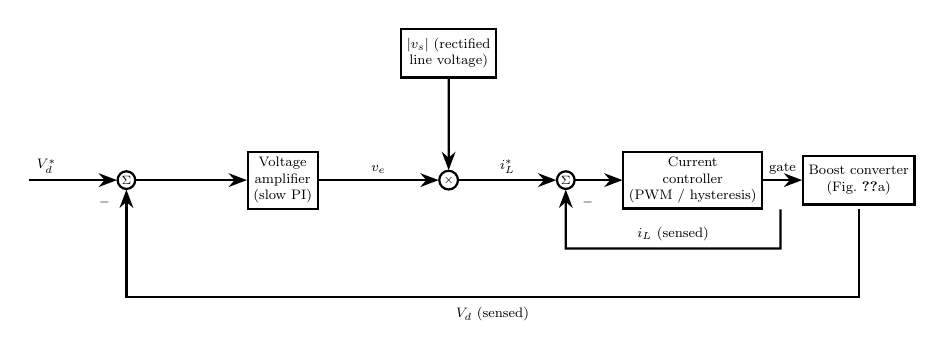
\begin{tikzpicture}[thick,scale=0.62,transform shape,>=Stealth,
   blk/.style={draw,thick,fill=white,minimum height=1.0cm,align=center,font=\footnotesize},
   sj/.style={draw,thick,circle,inner sep=1pt,font=\scriptsize}]
 \node[sj] (s1) at (0,0) {$\Sigma$};
 \node[blk] (gv) at (3.2,0) {Voltage\\amplifier\\(slow PI)};
 \node[sj] (mul) at (6.6,0) {$\times$};
 \node[blk] (vs) at (6.6,2.6) {$|v_s|$ (rectified\\line voltage)};
 \node[sj] (s2) at (9.0,0) {$\Sigma$};
 \node[blk] (gi) at (11.6,0) {Current\\controller\\(PWM / hysteresis)};
 \node[blk] (pw) at (15.0,0) {Boost converter\\(Fig.~\ref{fig:active_pfc}a)};
 \draw[->] (-2,0)--(s1) node[pos=0.2,above,font=\footnotesize]{$V_d^{*}$};
 \draw[->] (s1)--(gv); \draw[->] (gv)--(mul) node[midway,above,font=\footnotesize]{$v_e$};
 \draw[->] (vs)--(mul); \draw[->] (mul)--(s2) node[midway,above,font=\footnotesize]{$i_L^{*}$};
 \draw[->] (s2)--(gi); \draw[->] (gi)--(pw) node[midway,above,font=\footnotesize]{gate};
 \draw[->] (15.0,-0.6)--(15.0,-2.4)--(0,-2.4)--(s1);
 \node[font=\footnotesize] at (7.5,-2.75) {$V_d$ (sensed)};
 \draw[->] (13.4,-0.6)--(13.4,-1.4)--(9.0,-1.4)--(s2); \node[font=\footnotesize] at (11.2,-1.1) {$i_L$ (sensed)};
 \node[font=\scriptsize] at (-0.45,-0.45) {$-$}; \node[font=\scriptsize] at (9.45,-0.45) {$-$};
\end{tikzpicture}
\caption{Control architecture of the active PFC boost converter: slow outer voltage loop (regulates $V_d$, produces $v_e$), multiplier forming the reference $i_L^{*} = K v_e|v_s|$, and fast inner current loop driving the switch. (Redrawn; compare Mohan Fig.~18-5.)}
\label{fig:pfc_control}
\end{figure}

\subsubsection{Circuit Configuration and Dual-Loop Control Mechanics}
As depicted in Figures~\ref{fig:active_pfc} and~\ref{fig:pfc_control}, the active PFC step-up converter consists of a full-wave diode bridge, boost inductor $L$, power MOSFET/IGBT switch $S$, fast diode $D$, and DC bulk capacitor $C_d$.

The control system employs two cascaded feedback control loops:
\begin{enumerate}[leftmargin=*]
  \item \textbf{Slow Outer Voltage Loop (DC Bus Regulation):}
  \begin{itemize}
    \item Senses the DC link voltage $V_d$ and compares it to a precise reference $V_d^*$ (typically $390\text{ V} - 400\text{ V}$ DC for universal AC mains of $85\text{ V} - 265\text{ V}$).
    \item A proportional-integral (PI) voltage controller generates an error voltage signal $v_e$.
    \item \textbf{Deliberate Low Bandwidth:} The bandwidth of this loop is intentionally set very low ($10 - 20\text{ Hz}$) to prevent the controller from responding to the inevitable $100\text{ Hz}$ or $120\text{ Hz}$ ripple present on $V_d$.
  \end{itemize}

  \item \textbf{Analog Multiplier Stage:}
  \begin{itemize}
    \item Multiplies the slowly varying error signal $v_e$ with a rectified voltage template signal $|v_s(t)|$ obtained directly from a potential divider on the AC mains:
    \begin{equation}
    i_L^*(t) = K \cdot v_e \cdot |v_s(t)| = \hat{I}_L^* |\sin(\omega t)|
    \end{equation}
    This establishes an instantaneous reference current $i_L^*(t)$ that is guaranteed to have the exact same shape and phase as the AC mains voltage!
  \end{itemize}

  \item \textbf{Fast Inner Current Loop (Waveform Shaping):}
  \begin{itemize}
    \item Senses the instantaneous inductor current $i_L(t)$ using a shunt resistor or Hall-effect sensor.
    \item A high-bandwidth current controller (Average Current Mode Control or Peak Current Control) forces $i_L(t)$ to track $i_L^*(t)$ cycle-by-cycle at switching frequencies of $50 - 200\text{ kHz}$.
    \item When switch $S$ is closed: Inductor current rises ($di_L/dt = |v_s|/L$).
    \item When switch $S$ is open: Inductor current discharges into the load ($di_L/dt = (|v_s| - V_d)/L < 0$).
  \end{itemize}
\end{enumerate}

\subsubsection{Key Operating Metrics and Benefits of Active PFC}
\begin{itemize}[leftmargin=*]
  \item \textbf{Near-Unity Power Factor:} The input line current $i_s(t)$ is a clean, continuous sinusoid precisely in-phase with the line voltage ($\phi_1 \approx 0 \implies \text{DPF} \approx 1.0$).
  \item \textbf{Ultra-Low Harmonic Distortion:} $\text{THD}_i$ is suppressed from $>80\%$ down to $<3\% - 5\%$, easily satisfying IEEE 519 limits under all operating tiers!
  \item \textbf{Universal Input Voltage Range:} Active boost PFC automatically accommodates universal AC line inputs ($85\text{ V}_{\text{rms}} - 265\text{ V}_{\text{rms}}$, $47 - 63\text{ Hz}$) while maintaining a rock-steady regulated $400\text{ V}$ DC bus for downstream inverters or DC-DC stages!
\end{itemize}


\section{Ten Comprehensive University Exam Solved Numerical Problems}

\subsection{Problem 1: Single-Phase Full-Wave AC Voltage Controller with Resistive Load}
\begin{examplebox}[Problem 1: ACVC with $R$ Load Design \& Analysis]
\textbf{Statement:} A single-phase full-wave AC voltage controller is supplied from a $230\text{ V}$, $50\text{ Hz}$ single-phase source and feeds a purely resistive load of $R = 10\,\Omega$. The firing delay angle is set to $\alpha = \pi/3$ ($60^\circ$). Determine:
\begin{enumerate}
  \item The RMS output voltage $V_{or}$.
  \item The RMS load current $I_{or}$ and real active power dissipated in the load $P_o$.
  \item The input power factor $\text{PF}$.
  \item The average and RMS current ratings required for each individual thyristor.
\end{enumerate}

\tcblower
\textbf{Solution:}
\begin{enumerate}
  \item \textbf{RMS Output Voltage ($V_{or}$):}
  Using the master analytical formula for resistive load (equation~\eqref{eq:acvc_rms_r}):
  \begin{equation*}
  V_{or} = V_s \sqrt{1 - \frac{\alpha}{\pi} + \frac{\sin(2\alpha)}{2\pi}}
  \end{equation*}
  Here, $\alpha = \frac{\pi}{3} = 60^\circ$ ($1.0472\text{ rad}$), and $2\alpha = \frac{2\pi}{3} = 120^\circ$.
  \begin{equation*}
  \sin(2\alpha) = \sin(120^\circ) = \frac{\sqrt{3}}{2} \approx 0.8660
  \end{equation*}
  Substituting the numerical values into the square root expression:
  \begin{align*}
  \text{Term} &= 1 - \frac{\pi/3}{\pi} + \frac{0.8660}{2\pi} = 1 - \frac{1}{3} + \frac{0.8660}{6.2832} = \frac{2}{3} + 0.1378 = 0.6667 + 0.1378 = 0.8045 \notag\\
  \sqrt{0.8045} &\approx 0.8969
  \end{align*}
  Therefore, the RMS load voltage is:
  \begin{equation*}
  \mathbf{V_{or}} = 230 \times 0.8969 = \mathbf{206.3\text{ V}}
  \end{equation*}

  \item \textbf{RMS Load Current and Active Load Power:}
  \begin{equation*}
  \mathbf{I_{or}} = \frac{V_{or}}{R} = \frac{206.3\text{ V}}{10\,\Omega} = \mathbf{20.63\text{ A}}
  \end{equation*}
  The real power absorbed by the load resistor is:
  \begin{equation*}
  \mathbf{P_o} = I_{or}^2 \cdot R = (20.63)^2 \times 10 = \mathbf{4256\text{ W} = 4.256\text{ kW}}
  \end{equation*}

  \item \textbf{Input Power Factor ($\text{PF}$):}
  \begin{equation*}
  \mathbf{\text{PF}} = \frac{P_o}{V_s I_{or}} = \frac{V_{or}}{V_s} = \frac{206.3}{230} = \mathbf{0.897\text{ (lagging)}}
  \end{equation*}

  \item \textbf{Thyristor Current Ratings:}
  Each thyristor carries current for one half-cycle. Peak supply voltage is $V_m = \sqrt{2} \times 230 = 325.27\text{ V}$.
  \begin{align*}
  \mathbf{I_{T(avg)}} &= \frac{V_m}{2\pi R}(1 + \cos\alpha) = \frac{325.27}{2\pi \times 10}\left(1 + \cos 60^\circ\right) = \frac{32.527}{6.2832} (1 + 0.5) = 5.177 \times 1.5 = \mathbf{7.77\text{ A}} \notag\\
  \mathbf{I_{T(rms)}} &= \frac{I_{or}}{\sqrt{2}} = \frac{20.63}{\sqrt{2}} = \mathbf{14.59\text{ A}}
  \end{align*}
\end{enumerate}
\end{examplebox}

\subsection{Problem 2: Single-Phase AC Voltage Controller with Inductive $RL$ Load}
\begin{examplebox}[Problem 2: ACVC with $RL$ Load and Extinction Angle]
\textbf{Statement:} A $230\text{ V}$, $50\text{ Hz}$ single-phase AC voltage controller feeds a series $RL$ load with $R = 4\,\Omega$ and $\omega L = 3\,\Omega$.
\begin{enumerate}
  \item Determine the minimum permissible firing angle $\alpha_{\text{min}}$ for controllable operation.
  \item For a firing angle $\alpha = 60^\circ$, find the extinction angle $\beta$, the conduction angle $\gamma$ and the RMS output voltage $V_{or}$.
\end{enumerate}

\tcblower
\textbf{Solution:}
\begin{enumerate}
  \item \textbf{Minimum Firing Angle ($\alpha_{\text{min}}$):}
  \begin{align*}
  Z &= \sqrt{R^2 + (\omega L)^2} = \sqrt{4^2 + 3^2} = 5.0\,\Omega \notag\\
  \phi &= \arctan\left(\frac{\omega L}{R}\right) = \arctan\left(\frac{3}{4}\right) = 36.87^\circ = 0.6435\text{ rad}
  \end{align*}
  For independent phase control the delay angle must satisfy $\alpha \ge \phi$:
  \begin{equation*}
  \mathbf{\alpha_{\text{min}} = \phi = 36.87^\circ}
  \end{equation*}

  \item \textbf{Extinction angle $\beta$ (solve the transcendental equation).} With $\alpha = 60^\circ > \phi$ the current is discontinuous. $\beta$ is the first root beyond $\pi$ of
  \begin{align*}
  f(\beta) &= \sin(\beta - \phi) - \sin(\alpha - \phi)\,e^{-\frac{R}{\omega L}(\beta - \alpha)} = 0 \notag\\
  \sin(\alpha-\phi) &= \sin 23.13^\circ = 0.3928,\qquad \tfrac{R}{\omega L} = 1.3333
  \end{align*}
  Evaluate $f$ for two trial values and interpolate:
  \begin{align*}
  f(216^\circ) &= \sin(179.13^\circ) - 0.3928\,e^{-1.3333\times 2.7227} = 0.01518 - 0.01043 = +0.00476 \notag\\
  f(217^\circ) &= \sin(180.13^\circ) - 0.3928\,e^{-1.3333\times 2.7402} = -0.00227 - 0.01019 = -0.01246
  \end{align*}
  \begin{align*}
  \beta &\approx 216^\circ + \frac{0.00476}{0.00476 + 0.01246}\times 1^\circ \approx \mathbf{216.3^\circ} \notag\\
  \mathbf{\gamma} &= \beta - \alpha = \mathbf{156.3^\circ} = 2.728\text{ rad} \quad (<180^\circ:\ \text{discontinuous conduction})
  \end{align*}

  \item \textbf{RMS Output Voltage:} Using equation~\eqref{eq:acvc_rms_rl}:
  \begin{align*}
  2\beta &= 432.6^\circ = 72.6^\circ \implies \sin 2\beta = 0.9540, \qquad 2\alpha = 120^\circ \implies \sin 2\alpha = 0.8660 \notag\\
  \frac{\sin 2\beta - \sin 2\alpha}{2} &= \frac{0.9540 - 0.8660}{2} = 0.0440 \notag\\
  \frac{1}{\pi}\left[\gamma - 0.0440\right] &= \frac{2.728 - 0.044}{\pi} = 0.8543, \qquad \sqrt{0.8543} = 0.9243
  \end{align*}
  \begin{equation*}
  \mathbf{V_{or}} = 230 \times 0.9243 = \mathbf{212.6\text{ V}}
  \end{equation*}
  \textit{Check:} for a pure resistor at the same $\alpha$ the output would be $V_{or} = 230\sqrt{1 - \tfrac{1}{3} + \tfrac{\sin 120^\circ}{2\pi}} = 206.3\text{ V}$ (conduction $120^\circ$). The inductor keeps $T_1$ conducting for $156.3^\circ$ instead, so the $RL$ result $212.6\text{ V}$ is correctly larger.
\end{enumerate}
\end{examplebox}

\begin{figure}[htbp]
\centering
\includegraphics[width=0.78\textwidth]{fig_acvc_rl.pdf}
\caption{Problem 2 (computed from the exact solution): load voltage and current for $R = 4\,\Omega$, $\omega L = 3\,\Omega$, $\alpha = 60^\circ$. Conduction ends at $\beta = 216.3^\circ$; $i_o = 0$ until $T_2$ is fired at $\pi + \alpha = 240^\circ$.}
\label{fig:acvc_rl_problem}
\end{figure}

\subsection{Problem 3: Single-Phase Full-Bridge Square-Wave Inverter Analysis}
\begin{examplebox}[Problem 3: Square-Wave Full-Bridge Inverter Analysis]
\textbf{Statement:} A single-phase full-bridge inverter is fed from a $48\text{ V}$ battery bank and delivers power to a series $RL$ load with $R = 5\,\Omega$ and $L = 20\text{ mH}$ at fundamental frequency $f = 50\text{ Hz}$. Determine:
\begin{enumerate}
  \item The total RMS output voltage $V_{or}$ and the fundamental RMS output voltage $V_{o1(rms)}$.
  \item The fundamental load current $i_{o1}(t)$ and its RMS magnitude $I_{o1(rms)}$.
  \item The fundamental active power $P_1$ absorbed by the load.
  \item The total harmonic distortion of the output voltage $\text{THD}_v$.
  \item The exact steady-state load current: initial/peak value, zero-crossing instant, and the devices that conduct.
\end{enumerate}

\tcblower
\textbf{Solution:}
\begin{enumerate}
  \item \textbf{Output Voltages:}
  \begin{align*}
  \mathbf{V_{or}} &= V_{dc} = \mathbf{48.0\text{ V}} \notag\\
  \mathbf{V_{o1(rms)}} &= \frac{2\sqrt{2}}{\pi} V_{dc} = 0.9003 \times 48 = \mathbf{43.21\text{ V}}, \qquad \hat{V}_{o1} = \frac{4V_{dc}}{\pi} = 61.12\text{ V}
  \end{align*}

  \item \textbf{Fundamental Load Current:} $\omega = 2\pi \times 50 = 314.16\text{ rad/s}$.
  \begin{align*}
  X_{L1} &= \omega L = 314.16 \times 20 \times 10^{-3} = 6.283\,\Omega \notag\\
  Z_1 &= \sqrt{5^2 + 6.283^2} = 8.03\,\Omega, \qquad \phi_1 = \arctan\left(\frac{6.283}{5}\right) = 51.49^\circ
  \end{align*}
  \begin{equation*}
  \hat{I}_{o1} = \frac{61.12}{8.03} = 7.61\text{ A} \implies \mathbf{I_{o1(rms)}} = \frac{7.61}{\sqrt{2}} = \mathbf{5.38\text{ A}}, \qquad \mathbf{i_{o1}(t) = 7.61 \sin(314.16 t - 51.49^\circ)\text{ A}}
  \end{equation*}

  \item \textbf{Fundamental Active Power:}
  \begin{equation*}
  \mathbf{P_1} = I_{o1(rms)}^2 R = (5.38)^2 \times 5 \approx \mathbf{144.8\text{ W}}
  \end{equation*}

  \item \textbf{Total Harmonic Distortion of the voltage:}
  \begin{equation*}
  \mathbf{\text{THD}_v} = \sqrt{\left(\frac{V_{or}}{V_{o1(rms)}}\right)^2 - 1} = \sqrt{\left(\frac{48}{43.21}\right)^2 - 1} = \sqrt{1.2337 - 1} = \mathbf{48.34\%}
  \end{equation*}

  \item \textbf{Exact current (Eq.~\eqref{eq:vsi_rl_current}):} $\tau = L/R = 4\text{ ms}$, $T = 20\text{ ms}$, $\frac{T}{4\tau} = 1.25$, $\tanh 1.25 = 0.8483$.
  \begin{align*}
  I_0 &= -\frac{48}{5}\times 0.8483 = -8.14\text{ A}, \qquad I_{\max} = \mathbf{+8.14\text{ A}} \notag\\
  t_0 &= \tau\ln(1 + 0.8483) = 4\text{ ms}\times 0.614 = 2.46\text{ ms} \;\Longrightarrow\; \omega t_0 = \mathbf{44.2^\circ}
  \end{align*}
  For $0 < \omega t < 44.2^\circ$ the current is negative and flows through $D_1, D_2$ (energy returned to the battery); from $44.2^\circ$ to $180^\circ$ it flows through $S_1, S_2$; the second half-cycle repeats with $D_3, D_4$ and $S_3, S_4$. The exact RMS current is $5.44\text{ A}$ (total load power $148.1\text{ W}$); the harmonic currents are small ($3\text{rd}$: $1.05\text{ A}$ peak, $\text{THD}_i \approx 15\%$), which is why the fundamental analysis already gives $P \approx P_1$ within $2\%$.
\end{enumerate}
\end{examplebox}

\subsection{Problem 4: SPWM Full-Bridge Inverter with Bipolar Voltage Switching}
\begin{examplebox}[Problem 4: Bipolar SPWM Inverter Parameter Sizing]
\textbf{Statement:} A single-phase full-bridge inverter with sinusoidal PWM and bipolar switching is supplied from a $V_{dc} = 300\text{ V}$ DC rail. The carrier frequency is $f_s = 1.95\text{ kHz}$ and the output frequency is $f_o = 50\text{ Hz}$. The triangular carrier has amplitude $\hat{V}_{\text{tri}} = 5\text{ V}$ and the control reference has amplitude $\hat{V}_{\text{control}} = 4\text{ V}$.
\begin{enumerate}
  \item Determine $m_a$ and $m_f$.
  \item Calculate the peak and RMS fundamental output voltages.
  \item Identify the frequencies and peak amplitudes of the dominant harmonic components.
\end{enumerate}

\tcblower
\textbf{Solution:}
\begin{enumerate}
  \item \textbf{Modulation Indices:}
  \begin{align*}
  \mathbf{m_a} &= \frac{4\text{ V}}{5\text{ V}} = \mathbf{0.80} \notag\\
  \mathbf{m_f} &= \frac{f_s}{f_o} = \frac{1950}{50} = \mathbf{39}
  \end{align*}
  $m_f = 39$ is an odd integer (synchronous PWM, half-wave symmetry, no even harmonics), as required for bipolar switching.

  \item \textbf{Fundamental Output Voltages} ($m_a \le 1$: linear range):
  \begin{align*}
  \mathbf{\hat{V}_{o1}} &= m_a V_{dc} = 0.80 \times 300 = \mathbf{240.0\text{ V}} \notag\\
  \mathbf{V_{o1(rms)}} &= \frac{240}{\sqrt{2}} = \mathbf{169.7\text{ V}}
  \end{align*}

  \item \textbf{Dominant Harmonics} (Table~\ref{tab:mohan81}, column $m_a = 0.8$; peak value $= $ table entry $\times\, 300\text{ V}$):
  \begin{center}
  \begin{tabular}{l c c c}
  \toprule
  \textbf{Order} & \textbf{Frequency} & \textbf{Table entry} & \textbf{Peak amplitude} \\
  \midrule
  $m_f = 39$ & $1950\text{ Hz}$ & $0.818$ & $245.4\text{ V}$ \\
  $m_f \pm 2 = 37,\ 41$ & $1850\text{ Hz},\ 2050\text{ Hz}$ & $0.220$ & $66.0\text{ V}$ \\
  $2m_f \pm 1 = 77,\ 79$ & $3850\text{ Hz},\ 3950\text{ Hz}$ & $0.314$ & $94.2\text{ V}$ \\
  $2m_f \pm 3 = 75,\ 81$ & $3750\text{ Hz},\ 4050\text{ Hz}$ & $0.139$ & $41.7\text{ V}$ \\
  \bottomrule
  \end{tabular}
  \end{center}
  Notice that the carrier-frequency harmonic ($245\text{ V}$) is larger than the $240\text{ V}$ fundamental: it is removed by the output filter, not by the PWM.
\end{enumerate}
\end{examplebox}

\subsection{Problem 5: SPWM Full-Bridge Inverter with Unipolar Voltage Switching}
\begin{examplebox}[Problem 5: Unipolar Switching vs. Bipolar Output Filter Sizing]
\textbf{Statement:} The inverter of Problem 4 is reconfigured for \textbf{unipolar voltage switching} with the same $V_{dc} = 300\text{ V}$, $m_a = 0.80$, $f_o = 50\text{ Hz}$ and carrier frequency $f_s = 2\text{ kHz}$ ($m_f = 40$, even, as required for unipolar switching).
\begin{enumerate}
  \item Determine the peak and RMS fundamental output voltages.
  \item What is the lowest significant harmonic frequency in the unipolar output voltage?
  \item An $LC$ low-pass filter with corner frequency $f_c = \frac{1}{2\pi\sqrt{LC}}$ is placed one decade below the lowest significant harmonic. Compare the required $LC$ product for bipolar PWM (Problem 4) and unipolar PWM.
\end{enumerate}

\tcblower
\textbf{Solution:}
\begin{enumerate}
  \item \textbf{Fundamental Voltages} (identical to bipolar switching):
  \begin{equation*}
  \mathbf{\hat{V}_{o1}} = m_a V_{dc} = 0.80 \times 300 = \mathbf{240\text{ V}}, \qquad \mathbf{V_{o1(rms)}} = \frac{240}{\sqrt{2}} = \mathbf{169.7\text{ V}}
  \end{equation*}

  \item \textbf{Lowest Significant Harmonic:} all clusters at odd multiples of $m_f$ cancel; the first cluster is around $2m_f = 80$, with components at $2m_f \pm 1$ ($0.314\,V_{dc} = 94\text{ V}$) and $2m_f \pm 3$ ($0.139\,V_{dc} = 42\text{ V}$); the $2m_f \pm 5$ lines ($0.013\,V_{dc}$) are negligible. The lowest significant one is
  \begin{equation*}
  f_{\text{lowest}} = (2m_f - 3) f_o = 77 \times 50 = \mathbf{3850\text{ Hz}}
  \end{equation*}

  \item \textbf{$LC$ Filter Comparison:}
  \begin{itemize}
    \item \textbf{Bipolar} (Problem 4): the lowest significant harmonic is $(m_f - 2)f_o = 1850\text{ Hz}$. One decade below: $f_{c} = 185\text{ Hz}$:
    \begin{equation*}
    (LC)_{\text{bipolar}} = \frac{1}{(2\pi \times 185)^2} = \mathbf{7.40 \times 10^{-7}\text{ s}^2}
    \end{equation*}
    \item \textbf{Unipolar:} lowest significant harmonic $3850\text{ Hz}$; $f_{c} = 385\text{ Hz}$:
    \begin{equation*}
    (LC)_{\text{unipolar}} = \frac{1}{(2\pi \times 385)^2} = \mathbf{1.71 \times 10^{-7}\text{ s}^2}
    \end{equation*}
  \end{itemize}
  \textbf{Conclusion:} the ratio is $\approx 4.3$: doubling the frequency of the lowest harmonic cuts the $LC$ product to about \textbf{one quarter} (each of $L$ and $C$ about halved), reducing the weight, copper loss and cost of the filter.
\end{enumerate}
\end{examplebox}

\subsection{Problem 6: Three-Phase PWM Voltage Source Inverter}
\begin{examplebox}[Problem 6: Three-Phase SPWM Line-to-Line Voltage Calculation]
\textbf{Statement:} A three-phase bridge inverter is supplied from an electric vehicle battery pack of $V_{dc} = 400\text{ V}$. The inverter is controlled using three-phase sinusoidal PWM in the linear modulation range with $m_a = 0.85$ and $m_f = 21$.
\begin{enumerate}
  \item Calculate the peak and RMS values of the fundamental phase-to-neutral (pole) voltage.
  \item Calculate the peak and RMS values of the fundamental line-to-line output voltage.
  \item Calculate the maximum achievable RMS fundamental line-to-line voltage in the linear range ($m_a = 1.0$), and compare it to the six-step square-wave mode.
\end{enumerate}

\tcblower
\textbf{Solution:}
\begin{enumerate}
  \item \textbf{Fundamental Phase Voltage ($v_{Ao1}$):}
  \begin{align*}
  \mathbf{\hat{V}_{Ao1}} &= m_a \frac{V_{dc}}{2} = 0.85 \times \frac{400}{2} = \mathbf{170.0\text{ V}} \notag\\
  \mathbf{V_{Ao1(rms)}} &= \frac{\hat{V}_{Ao1}}{\sqrt{2}} = \frac{170}{\sqrt{2}} = \mathbf{120.2\text{ V}}
  \end{align*}

  \item \textbf{Fundamental Line-to-Line Voltage ($V_{LL1}$):}
  Using equations~\eqref{eq:vll1_peak} and~\eqref{eq:vll1_rms}:
  \begin{align*}
  \mathbf{\hat{V}_{LL1}} &= \sqrt{3} \hat{V}_{Ao1} = \sqrt{3} \times 170.0\text{ V} = \mathbf{294.4\text{ V}} \notag\\
  \mathbf{V_{LL1(rms)}} &= \frac{\sqrt{6}}{4} m_a V_{dc} = 0.6124 \times 0.85 \times 400 = \mathbf{208.2\text{ V}}
  \end{align*}

  \item \textbf{Maximum Voltage Comparison:}
  \begin{itemize}
    \item \textbf{Maximum Linear SPWM ($m_a = 1.0$):}
    \begin{equation*}
    V_{LL1(rms),\text{max}} = 0.6124 \times 400\text{ V} = \mathbf{245.0\text{ V}}
    \end{equation*}
    \item \textbf{Six-Step Square-Wave Mode:}
    \begin{equation*}
    V_{LL1(rms),\text{square}} = \frac{\sqrt{6}}{\pi} V_{dc} = \frac{\sqrt{6}}{\pi} \times 400 = 0.7797 \times 400 = \mathbf{311.9\text{ V}}
    \end{equation*}
  \end{itemize}
  Operating in six-step mode yields $\frac{311.9}{245.0} = 1.273$ ($+27.3\%$) higher fundamental voltage than linear SPWM.
\end{enumerate}
\end{examplebox}

\subsection{Problem 7: Third Harmonic Injection PWM (THIPWM) Voltage Boost}
\begin{examplebox}[Problem 7: THIPWM DC Bus Utilization Advantage]
\textbf{Statement:} A three-phase inverter fed from a $V_{dc} = 600\text{ V}$ DC bus supplies a $415\text{ V}$ (RMS line-to-line), $50\text{ Hz}$ induction motor.
\begin{enumerate}
  \item Can standard sinusoidal PWM in the linear range deliver $415\text{ V}$?
  \item What is the maximum line-to-line RMS voltage with third-harmonic-injection PWM while staying in the linear range?
  \item Can THIPWM supply the motor at rated voltage without over-modulation? What are the required $m_a$ and the peak of the composite reference?
\end{enumerate}

\tcblower
\textbf{Solution:}
\begin{enumerate}
  \item \textbf{Standard SPWM:} the linear limit is $m_a = 1.0$:
  \begin{equation*}
  V_{LL1(rms),\text{max (SPWM)}} = 0.6124 \times 600 = \mathbf{367.4\text{ V}}
  \end{equation*}
  Since $367.4\text{ V} < 415\text{ V}$, SPWM cannot give rated voltage in the linear range (it would need $m_a = 415/367.4 = 1.13$, i.e.\ over-modulation with low-order harmonics).

  \item \textbf{THIPWM:} the fundamental index may rise to $\frac{2}{\sqrt{3}} = 1.1547$:
  \begin{equation*}
  V_{LL1(rms),\text{max (THIPWM)}} = 0.6124 \times 1.1547 \times 600 = \frac{V_{dc}}{\sqrt{2}} = \mathbf{424.3\text{ V}}
  \end{equation*}

  \item \textbf{Feasibility:} $424.3\text{ V} > 415\text{ V}$, so THIPWM can supply the motor. The fundamental index required is
  \begin{equation*}
  m_a = \frac{415}{0.6124 \times 600} = \mathbf{1.129} \;(\le 1.1547)
  \end{equation*}
  Although $m_a > 1$, there is no over-modulation: the composite reference $\hat{V}_1\left[\sin\omega t + \frac{1}{6}\sin 3\omega t\right]$ peaks at $0.866 \times 1.129 = \mathbf{0.978}$ of the carrier amplitude, which is below $1$. The motor voltage therefore stays sinusoidal and free of low-order harmonics, with a $2.2\%$ voltage margin.
\end{enumerate}
\end{examplebox}

\subsection{Problem 8: Analytical Evaluation of Dead-Time (Blanking Time) Voltage Error}
\begin{examplebox}[Problem 8: Dead-Time Induced Fundamental Voltage Reduction]
\textbf{Statement:} A three-phase IGBT inverter operates from a $V_{dc} = 750\text{ V}$ DC bus at a switching frequency $f_s = 10\text{ kHz}$ with a programmed blanking time $t_d = 2.5\,\mu\text{s}$.
\begin{enumerate}
  \item Calculate the average pole-voltage error $\Delta V_{Ao}$ of one phase leg.
  \item Determine the percentage reduction of the fundamental voltage at modulation index $m_a = 0.20$ (low-speed operation), assuming the phase current is in phase with the fundamental voltage.
  \item Propose a compensation method for a DSP-controlled drive.
\end{enumerate}

\tcblower
\textbf{Solution:}
\begin{enumerate}
  \item \textbf{Average pole-voltage error:} using equation~\eqref{eq:deadtime_voltage_drop},
  \begin{equation*}
  |\Delta V_{Ao}| = f_s\,t_d\,V_{dc} = (10\times 10^{3})(2.5\times 10^{-6})(750) = 0.025 \times 750 = \mathbf{18.75\text{ V}}
  \end{equation*}
  i.e.\ $t_d/T_s = 2.5\%$ of $V_{dc}$, with a sign opposite to the current: $-18.75\text{ V}$ for $i_A > 0$ and $+18.75\text{ V}$ for $i_A < 0$.

  \item \textbf{Effect on the fundamental at $m_a = 0.20$:} the nominal peak fundamental pole voltage is
  \begin{equation*}
  \hat{V}_{Ao1} = m_a\frac{V_{dc}}{2} = 0.20 \times \frac{750}{2} = 75.0\text{ V}
  \end{equation*}
  The error is a square wave of amplitude $18.75\text{ V}$ in phase with $\operatorname{sgn}(i_A)$; its fundamental has peak
  \begin{equation*}
  \hat{V}_{\text{error},1} = \frac{4}{\pi}\,(f_s t_d V_{dc}) = \frac{4}{\pi}\times 18.75 = 23.87\text{ V}
  \end{equation*}
  \begin{equation*}
  \text{Loss} = \frac{23.87}{75.0}\times 100\% = \mathbf{31.8\%}
  \end{equation*}
  Almost one third of the commanded voltage is lost at low speed. The error is a fixed voltage, so its relative effect grows as $m_a$ falls; the square wave also contains 5th and 7th harmonics that produce torque pulsation. (With a lagging current the error vector is rotated with the current, adding a phase error as well.)

  \item \textbf{Compensation:} the DSP senses the sign of each phase current and adds $+f_s t_d V_{dc} = 18.75\text{ V}$ to the voltage reference of leg $A$ when $i_A > 0$ (and $-18.75\text{ V}$ when $i_A < 0$), equivalently shifts the PWM compare value by $t_d$. Near the current zero crossing the sign is uncertain, so practical schemes smooth the correction over a small current band.
\end{enumerate}
\end{examplebox}

\subsection{Problem 9: Power Factor and THD in Non-Sinusoidal Rectifiers}
\begin{examplebox}[Problem 9: True Power Factor and Distortion Factor Evaluation]
\textbf{Statement:} A single-phase diode bridge rectifier with a capacitive filter draws a non-sinusoidal input current from a $230\text{ V}$, $50\text{ Hz}$ supply. A power quality analyzer records the fundamental current component as $I_{s1} = 10\text{ A}$ (RMS) lagging the line voltage by $\phi_1 = 18^\circ$, and harmonic current components of: $I_{s3} = 7.5\text{ A}$, $I_{s5} = 4.5\text{ A}$, $I_{s7} = 2.0\text{ A}$, and $I_{s9} = 1.0\text{ A}$ (higher harmonics negligible).
\begin{enumerate}
  \item Calculate the total RMS input current $I_s$.
  \item Compute the current Total Harmonic Distortion ($\text{THD}_i$).
  \item Determine the Distortion Factor ($K_{\text{dist}}$) and Displacement Power Factor ($\text{DPF}$).
  \item Calculate the True Power Factor ($\text{PF}$) and real active power drawn from the mains.
\end{enumerate}

\tcblower
\textbf{Solution:}
\begin{enumerate}
  \item \textbf{Total RMS Current ($I_s$):}
  \begin{align*}
  I_{\text{dist}}^2 &= \sum_{h=3,5,7,9} I_{sh}^2 = (7.5)^2 + (4.5)^2 + (2.0)^2 + (1.0)^2 = 56.25 + 20.25 + 4.0 + 1.0 = 81.5\text{ A}^2 \notag\\
  I_s &= \sqrt{I_{s1}^2 + I_{\text{dist}}^2} = \sqrt{10^2 + 81.5} = \sqrt{181.5} = \mathbf{13.47\text{ A}}
  \end{align*}

  \item \textbf{Current Total Harmonic Distortion ($\text{THD}_i$):}
  \begin{equation*}
  \mathbf{\text{THD}_i} = \frac{\sqrt{I_{\text{dist}}^2}}{I_{s1}} = \frac{\sqrt{81.5}}{10} = \frac{9.028}{10} = 0.9028 \implies \mathbf{90.28\%}
  \end{equation*}

  \item \textbf{Distortion Factor and Displacement Factor:}
  \begin{align*}
  \mathbf{K_{\text{dist}}} &= \frac{I_{s1}}{I_s} = \frac{10\text{ A}}{13.47\text{ A}} = \mathbf{0.7424} \notag\\
  \mathbf{\text{DPF}} &= \cos\phi_1 = \cos(18^\circ) = \mathbf{0.9511}
  \end{align*}

  \item \textbf{True Power Factor and Real Power:}
  Using equation~\eqref{eq:true_pf}:
  \begin{equation*}
  \mathbf{\text{PF}} = K_{\text{dist}} \times \text{DPF} = 0.7424 \times 0.9511 = \mathbf{0.706\text{ (lagging)}}
  \end{equation*}
  Verification using equation~\eqref{eq:pf_from_thd}:
  \begin{equation*}
  \text{PF} = \frac{\cos(18^\circ)}{\sqrt{1 + (0.9028)^2}} = \frac{0.9511}{\sqrt{1 + 0.815}} = \frac{0.9511}{\sqrt{1.815}} = \frac{0.9511}{1.3472} = 0.706\text{ (Exact match!)}
  \end{equation*}
  Real active power consumed:
  \begin{equation*}
  \mathbf{P} = V_s I_{s1} \cos\phi_1 = 230 \times 10 \times 0.9511 = \mathbf{2187.5\text{ W} = 2.188\text{ kW}}
  \end{equation*}
  Apparent power: $S = V_s I_s = 230 \times 13.47 = 3098\text{ VA}$. $\text{PF} = 2187.5 / 3098 = 0.706$.
\end{enumerate}
\end{examplebox}

\subsection{Problem 10: Active Power Factor Correction (PFC) Boost Converter Design}
\begin{examplebox}[Problem 10: Active PFC Boost Inductor Sizing \& IEEE 519 Check]
\textbf{Statement:} A $1.5\text{ kW}$ single-phase Active PFC boost converter is connected to a $230\text{ V}_{\text{rms}}$, $50\text{ Hz}$ AC line. The regulated DC bus voltage is $V_d = 400\text{ V}$, switching frequency is $f_s = 100\text{ kHz}$, and target converter efficiency is $\eta = 95\%$.
\begin{enumerate}
  \item Determine the peak and RMS fundamental input currents drawn from the AC line.
  \item Calculate the maximum peak-to-peak inductor ripple current $\Delta I_{L,\text{max}}$ if ripple is limited to $20\%$ of peak input current.
  \item Calculate the required boost inductance $L$.
  \item At the customer Point of Common Coupling (PCC), the available short-circuit current is $I_{sc} = 650\text{ A}$. What is the maximum permissible total demand distortion (TDD) specified by IEEE 519?
\end{enumerate}

\tcblower
\textbf{Solution:}
\begin{enumerate}
  \item \textbf{Input Line Currents:}
  Input active power drawn from the mains:
  \begin{equation*}
  P_{\text{in}} = \frac{P_{\text{out}}}{\eta} = \frac{1500\text{ W}}{0.95} = 1578.9\text{ W}
  \end{equation*}
  Since the PFC converter shapes current to achieve near-unity power factor ($\text{PF} \approx 1.0$):
  \begin{align*}
  \mathbf{I_{s(rms)}} &= \frac{P_{\text{in}}}{V_s} = \frac{1578.9\text{ W}}{230\text{ V}} = \mathbf{6.86\text{ A}} \notag\\
  \mathbf{\hat{I}_s} &= \sqrt{2} \times I_{s(rms)} = \sqrt{2} \times 6.86 = \mathbf{9.71\text{ A}}
  \end{align*}

  \item \textbf{Maximum Inductor Ripple Current ($\Delta I_{L,\text{max}}$):}
  \begin{equation*}
  \Delta I_{L,\text{max}} = 20\% \times \hat{I}_s = 0.20 \times 9.71\text{ A} = \mathbf{1.942\text{ A}}
  \end{equation*}

  \item \textbf{Boost Inductance Sizing ($L$):}
  In a boost PFC converter, the duty cycle varies continuously across the line cycle: $d(t) = 1 - \frac{|v_s(t)|}{V_d}$. The ripple current is:
  \begin{equation*}
  \Delta i_L = \frac{|v_s| \cdot d}{f_s L} = \frac{|v_s|}{f_s L} \left(1 - \frac{|v_s|}{V_d}\right)
  \end{equation*}
  Differentiating with respect to $|v_s|$ shows that maximum ripple occurs precisely when $|v_s| = \frac{V_d}{2} = \frac{400}{2} = 200\text{ V}$ (where duty cycle $d = 0.5$):
  \begin{equation*}
  \Delta I_{L,\text{max}} = \frac{V_d / 2 \cdot 0.5}{f_s L} = \frac{V_d}{4 f_s L}
  \end{equation*}
  Rearranging to solve for inductance $L$:
  \begin{align*}
  \mathbf{L} &= \frac{V_d}{4 f_s \Delta I_{L,\text{max}}} = \frac{400\text{ V}}{4 \times (100 \times 10^3\text{ Hz}) \times 1.942\text{ A}} \notag\\
  &= \frac{400}{776,800} = 5.15 \times 10^{-4}\text{ H} = \mathbf{0.515\text{ mH} \approx 520\,\mu\text{H}}
  \end{align*}

  \item \textbf{IEEE 519 TDD Limit Evaluation:}
  The maximum fundamental load current is $I_L = I_{s(rms)} = 6.86\text{ A}$. The Short-Circuit Ratio (SCR) at the PCC is:
  \begin{equation*}
  \mathbf{\text{SCR}} = \frac{I_{sc}}{I_L} = \frac{650\text{ A}}{6.86\text{ A}} = \mathbf{94.75}
  \end{equation*}
  From Table~\ref{tab:ieee519_limits}, for $50 < \frac{I_{sc}}{I_L} < 100$:
  \begin{equation*}
  \mathbf{\text{Maximum Permissible TDD}} = \mathbf{12.0\%}
  \end{equation*}
  Since active PFC achieves $\text{THD}_i < 5\%$, the installation effortlessly complies with IEEE 519 with massive safety margins!
\end{enumerate}
\end{examplebox}


\section{Master Formula Sheet \& Quick Revision Tables}

\subsection{Master Analytical Formula Matrix}

\begin{table}[htbp]
\centering
\small
\caption{Module 3 Master Analytical Formula Cheat-Sheet for Fast Exam Revision: ACVC and single-phase inverters}
\label{tab:module3_master_formulas}
\begin{tabularx}{\textwidth}{l p{5.5cm} X}
\toprule
\textbf{Topic / Circuit} & \textbf{Key Formulas / Governing Equations} & \textbf{Exam Tips \& Critical Insights} \\
\midrule
\textbf{ACVC ($R$ Load)} &
$V_{or} = V_s \sqrt{1 - \frac{\alpha}{\pi} + \frac{\sin 2\alpha}{2\pi}}$ \newline
$\text{PF} = \frac{V_{or}}{V_s} = \sqrt{1 - \frac{\alpha}{\pi} + \frac{\sin 2\alpha}{2\pi}}$ &
At $\alpha=0 \implies V_{or}=V_s, \text{PF}=1.0$. \newline
At $\alpha=90^\circ \implies V_{or}=0.707 V_s, \text{PF}=0.707$. \newline
At $\alpha=180^\circ \implies V_{or}=0, \text{PF}=0$. \\
\midrule
\textbf{ACVC ($RL$ Load)} &
$i_o(\omega t) = \frac{V_m}{Z}[\sin(\omega t-\phi) - \sin(\alpha-\phi)e^{-\frac{R}{\omega L}(\omega t-\alpha)}]$ \newline
$\sin(\beta-\phi) = \sin(\alpha-\phi)e^{-\frac{R}{\omega L}(\beta-\alpha)}$ \newline
$V_{or} = V_s \sqrt{\frac{1}{\pi}[(\beta-\alpha) - \frac{\sin 2\beta - \sin 2\alpha}{2}]}$ &
\textbf{Rule:} $\alpha \ge \phi = \arctan(\omega L / R)$. \newline
If $\alpha = \phi \implies \beta = \pi + \alpha \implies \gamma = 180^\circ$ (continuous sinusoidal current). \newline
Requires high-frequency pulse train gating! \\
\midrule
\textbf{ACVC (Integral Cycle)} &
$k = \frac{n}{n+m}$, \quad $V_{or} = V_s \sqrt{k}$ \newline
$\text{PF} = \sqrt{k}$ &
Zero switching EMI ($dv/dt=0, di/dt=0$). \newline
Causes line flicker/sub-harmonics. Used for thermal loads. \\
\midrule
\textbf{Half-Bridge VSI (Square Wave)} &
$v_o = \pm V_{dc}/2$, \quad $V_{or} = V_{dc}/2$ \newline
$\hat{V}_{o1} = \frac{2}{\pi}V_{dc}$, \quad $V_{o1(rms)} = \frac{\sqrt{2}}{\pi}V_{dc} \approx 0.45 V_{dc}$ &
Requires 3-wire DC split supply. \newline
Switch voltage rating $= V_{dc}$ ($2 \times$ peak output). \\
\midrule
\textbf{Full-Bridge VSI (Square Wave)} &
$v_o = \pm V_{dc}$, \quad $V_{or} = V_{dc}$ \newline
$\hat{V}_{o1} = \frac{4}{\pi}V_{dc}$, \quad $V_{o1(rms)} = \frac{2\sqrt{2}}{\pi}V_{dc} \approx 0.90 V_{dc}$ \newline
$\text{THD}_v = \sqrt{\frac{\pi^2}{8}-1} = 48.34\%$ &
Odd harmonics only ($n=1, 3, 5, 7, \dots$). \newline
Harmonic amplitude $\hat{V}_{on} = \hat{V}_{o1}/n$. \newline
Twice the voltage, $4\times$ power of half-bridge! \\
\midrule
\textbf{Full-Bridge VSI, $RL$ load} &
$I_0 = -\frac{V_{dc}}{R}\tanh\frac{T}{4\tau}$, \quad $t_0 = \tau\ln\left(1 + \tanh\frac{T}{4\tau}\right)$ \newline
$i_o = \sum \frac{4V_{dc}}{n\pi Z_n}\sin(n\omega t - \phi_n)$ &
Current is negative for $0<t<t_0$ although $v_o = +V_{dc}$: carried by feedback diodes $D_1, D_2$. \newline
Sequence: $D_1D_2 \to S_1S_2 \to D_3D_4 \to S_3S_4$. \\
\midrule
\textbf{Single-Pulse PWM} &
$V_{or} = V_{dc}\sqrt{\delta/\pi}$ \newline
$\hat{V}_{o1} = \frac{4V_{dc}}{\pi}\sin\frac{\delta}{2}$, \quad $v_{on} \propto \sin\frac{n\delta}{2}$ &
$\delta = 120^\circ$ removes the 3rd, $72^\circ$ the 5th harmonic. \newline
Only one harmonic can be eliminated at a time. \\
\midrule
\textbf{Single-Phase Bipolar SPWM} &
$m_a = \frac{\hat{V}_{\text{control}}}{\hat{V}_{\text{tri}}}$, \quad $m_f = \frac{f_s}{f_o}$ \newline
$\hat{V}_{o1} = m_a V_{dc}$, \quad $V_{o1(rms)} = \frac{m_a V_{dc}}{\sqrt{2}}$ &
$m_f$ must be an odd integer (eliminates even harmonics). \newline
Lowest harmonics clustered at $m_f \pm 2$. \\
\midrule
\textbf{Single-Phase Unipolar SPWM} &
$\hat{V}_{o1} = m_a V_{dc}$, \quad $V_{o1(rms)} = \frac{m_a V_{dc}}{\sqrt{2}}$ \newline
Effective switching frequency $= 2f_s$ &
3-level output ($+V_{dc}, 0, -V_{dc}$). \newline
Harmonics around $m_f$ cancel! First cluster at $2m_f$. \newline
$LC$ product reduced to about $\frac{1}{4}$ ($L$, $C$ each $\approx$ halved). \\
\bottomrule
\end{tabularx}
\end{table}

\begin{table}[htbp]
\centering
\small
\caption{Module 3 Master Analytical Formula Cheat-Sheet (continued): three-phase inverters, dead time, harmonics and PFC}
\label{tab:module3_master_formulas_b}
\begin{tabularx}{\textwidth}{l p{5.5cm} X}
\toprule
\textbf{Topic / Circuit} & \textbf{Key Formulas / Governing Equations} & \textbf{Exam Tips \& Critical Insights} \\
\midrule
\textbf{Three-Phase SPWM (Linear)} &
$\hat{V}_{Ao1} = m_a \frac{V_{dc}}{2}$ \newline
$\hat{V}_{LL1} = \frac{\sqrt{3}}{2} m_a V_{dc} \approx 0.866 m_a V_{dc}$ \newline
$V_{LL1(rms)} = \frac{\sqrt{6}}{4} m_a V_{dc} \approx 0.6124 m_a V_{dc}$ &
Triplen harmonics (3rd, 9th, 15th, \dots) cancel in line-line! \newline
Choose $m_f$ as an odd multiple of 3 ($9, 15, 21, \dots$). \newline
Max linear RMS line voltage $= 0.6124 V_{dc}$. \\
\midrule
\textbf{Three-Phase Six-Step (Square)} &
$V_{LL(rms)} = \sqrt{\frac{2}{3}}V_{dc} \approx 0.8165 V_{dc}$ \newline
$V_{LL1(rms)} = \frac{\sqrt{6}}{\pi}V_{dc} \approx 0.7797 V_{dc}$ &
$180^\circ$ conduction. Output contains $n=6k \pm 1$ ($5th, 7th, 11th$). \newline
Fundamental is $27.3\%$ higher than max linear SPWM. \\
\midrule
\textbf{Third Harmonic Injection (THIPWM)} &
$v_{\text{control}} = \hat{V}_1 [\sin(\omega t) + \frac{1}{6}\sin(3\omega t)]$ \newline
$V_{LL1(rms),\text{max}} = \frac{V_{dc}}{\sqrt{2}} \approx 0.707 V_{dc}$ &
Composite reference peaks at only $0.866\hat{V}_1$ (at $60^\circ, 120^\circ$), so $m_a$ may reach $1.1547$. \newline
\textbf{Boosts linear output voltage by 15.5\%!} \newline
Third harmonic cancels out in line-to-line output! \\
\midrule
\textbf{Blanking Time (Dead-Time)} &
$|\Delta V_{Ao}| = \frac{t_d}{T_s}V_{dc} = f_s t_d V_{dc}$ per leg, sign opposite to $i_A$ \newline
Single-phase bipolar bridge: $|\Delta V_o| = 2 f_s t_d V_{dc}$ \newline
Fundamental of error: $\frac{4}{\pi} f_s t_d V_{dc}$ (peak, per leg) &
Prevents DC-link shoot-through. \newline
Pulse shorter by $t_d$ for $i_o>0$, longer for $i_o<0$. \newline
Worst at low $m_a$; causes 5th/7th harmonics. \\
\midrule
\textbf{Harmonics \& Power Factor} &
$\text{PF} = \left(\frac{I_{s1}}{I_s}\right) \cos\phi_1 = \frac{\cos\phi_1}{\sqrt{1 + \text{THD}_i^2}}$ \newline
$\text{THD}_i = \frac{\sqrt{I_s^2 - I_{s1}^2}}{I_{s1}}$ &
True PF $=$ Distortion Factor $\times$ Displacement Factor. \newline
Harmonics alone reduce power factor even if $\cos\phi_1 = 1.0$! \\
\midrule
\textbf{Active PFC Boost Inductor} &
$\Delta I_{L,\text{max}} = \frac{V_d}{4 f_s L} \implies L = \frac{V_d}{4 f_s \Delta I_{L,\text{max}}}$ &
Max ripple occurs at $d=0.5$ ($|v_s| = V_d/2$). \newline
Universal AC input, regulates $V_d \approx 400\text{ V}$ DC, $\text{THD}_i < 5\%$. \\
\bottomrule
\end{tabularx}
\end{table}

\subsection{Essential Examination Quick-Tips for KTU S5 EEE Students}
\begin{enumerate}[leftmargin=*]
  \item \textbf{When asked for ACVC RMS Voltage Derivation:} Always state the half-wave symmetry condition ($v_o(\omega t + \pi) = -v_o(\omega t)$), integrate $[V_m \sin\omega t]^2$ from $\alpha$ to $\pi$ (or $\alpha$ to $\beta$ for $RL$ load), convert $\sin^2\theta = \frac{1 - \cos 2\theta}{2}$, and show every intermediate integration step clearly to secure full marks.
  \item \textbf{Why $\alpha < \phi$ is prohibited in $RL$ ACVC:} Remember the physical mechanism: If $\alpha < \phi$, the current in the previous thyristor is still flowing when the next thyristor is triggered. Conduction becomes continuous, phase control is lost ($V_{or} = V_s$ for every $\alpha < \phi$ with long gate pulses), and the thyristors behave as if the load were connected directly to the AC mains. With narrow gate pulses one thyristor may not fire at all, giving a unidirectional (DC-offset) current.
  \item \textbf{Fourier Series of Square Wave Inverter:} Write down the general half-wave symmetry property first. State why all even harmonics and DC term are zero ($a_0 = 0, a_n = 0, b_{\text{even}} = 0$). Write the general formula $\sum \frac{4V_{dc}}{n\pi}\sin(n\omega t)$ and calculate $\text{THD}_v = \sqrt{\frac{\pi^2}{8}-1} = 48.34\%$.
  \item \textbf{Bipolar vs. Unipolar PWM Comparison:} Draw the two-level vs. three-level output waveforms side-by-side. Highlight the three killer facts: (1) Effective switching frequency doubles to $2f_s$; (2) Harmonics around $m_f$ cancel out completely; (3) The $LC$ product of the output filter falls to about $\frac{1}{4}$ ($L$ and $C$ each about halved).
  \item \textbf{Why Triplen Harmonics Disappear in 3-Phase Inverters:} State that triplen harmonics (3rd, 9th, 15th, \dots) form a zero-sequence set—they are exactly equal in magnitude and in phase in all three inverter legs ($v_{Ao,3} = v_{Bo,3} = v_{Co,3}$). When computing line-to-line voltage $v_{AB} = v_{Ao} - v_{Bo}$, they subtract to exactly zero!
  \item \textbf{Dead-Time Derivation:} Draw the leg diagram showing $S_1, S_4$ and diodes $D_1, D_4$. Explain that when both switches are off during $t_d$, the load current $i_o$ forces either $D_1$ or $D_4$ to conduct depending solely on the sign of $i_o$, subtracting or adding $V_{dc}t_d$ of volt-seconds to the output pulse. The average pole-voltage error is $\frac{t_d}{T_s}V_{dc} = f_s t_d V_{dc}$ (not $4 f_s t_d V_{dc}$; the $\frac{4}{\pi}$ appears only in the fundamental of the error square wave).
  \item \textbf{IEEE 519 PCC Rule:} Remember that IEEE 519 applies strictly at the \textbf{Point of Common Coupling (PCC)}, NOT inside the customer plant. Limits are specified in terms of \textbf{Total Demand Distortion (TDD)} and depend directly on the short-circuit ratio $I_{sc} / I_L$.
\end{enumerate}

\subsection{Short-Answer Drill (Part-A style, 3 marks each)}
\begin{enumerate}[leftmargin=*]
  \item \textbf{State the RMS output voltage of a single-phase full-wave ACVC with $R$ load.} $V_{or} = V_s\sqrt{1 - \frac{\alpha}{\pi} + \frac{\sin 2\alpha}{2\pi}}$; it falls from $V_s$ at $\alpha = 0$ to $0.707V_s$ at $90^\circ$ and $0$ at $180^\circ$.
  \item \textbf{Why is a high-frequency pulse train used to gate the thyristors of an $RL$ ACVC?} If the first pulse arrives while the load current has not yet fallen to zero (or while the thyristor is not yet forward-biased), the thyristor would not latch; a pulse train keeps re-triggering until it does.
  \item \textbf{Define $m_a$ and $m_f$.} $m_a = \hat{V}_{control}/\hat{V}_{tri}$ sets the fundamental, $\hat{V}_{o1} = m_aV_{dc}$ for $m_a \le 1$; $m_f = f_s/f_o$ sets where the harmonics appear.
  \item \textbf{Why must $m_f$ be odd (bipolar) and odd and a multiple of 3 (three-phase)?} Odd $m_f$ gives half-wave symmetry and removes even harmonics; a multiple of 3 makes the $m_f$ harmonic identical in the three legs so it cancels in the line voltage.
  \item \textbf{What are the advantages of unipolar over bipolar switching?} Three output levels, the output pulse frequency is $2f_s$, harmonics around $m_f$ are cancelled (first cluster at $2m_f$), current ripple and filter size are smaller, and the $dv/dt$ step is $V_{dc}$ instead of $2V_{dc}$.
  \item \textbf{Why is blanking time needed, and what is its drawback?} It prevents shoot-through of the two switches of a leg ($t_{off} > t_{on}$). It makes the pole voltage depend on the current sign, so the output is reduced by about $f_st_dV_{dc}$ per leg and low-order harmonics appear.
  \item \textbf{What happens in the over-modulation region?} $m_a > 1$: pulses are dropped, $\hat{V}_{o1}$ grows non-linearly towards $\frac{4V_{dc}}{\pi}$ and low-order harmonics appear.
  \item \textbf{How does third-harmonic injection raise the output voltage?} Adding $\frac{1}{6}\sin 3\omega t$ lowers the peak of the reference to $0.866$ of its fundamental, so the fundamental can be raised by $1.1547$ (15.5\%) with no over-modulation. The third harmonic is zero-sequence and cancels in the line voltage.
  \item \textbf{Compare a VSI and a CSI.} A VSI has a stiff DC voltage source: output voltage imposed by the switches, current by the load, anti-parallel diodes needed, shoot-through is fatal, an open circuit is harmless. A CSI has a stiff DC current source ($L_{dc}$): output current imposed by the switches, voltage by the load, series blocking diodes needed, simultaneous conduction in a leg is harmless, an open circuit is fatal.
  \item \textbf{Define displacement factor, distortion factor and power factor of a non-sinusoidal current.} DPF $= \cos\phi_1$; distortion factor $= I_{s1}/I_s = 1/\sqrt{1 + \text{THD}_i^2}$; $\text{PF} = I_{s1}\cos\phi_1/I_s$.
  \item \textbf{What does IEEE 519 limit, and where?} Harmonic current (as TDD, with limits depending on $I_{sc}/I_L$) and harmonic voltage (THD$_v$ and individual) at the PCC.
  \item \textbf{How does an active PFC boost converter shape the input current?} An outer slow loop regulates $V_d$; its output multiplies $|v_s|$ to give $i_L^* = Kv_e|v_s|$; a fast inner loop forces the boost inductor current $i_L$ to follow $i_L^*$, so the input current is a sinusoid in phase with the line voltage.
\end{enumerate}

\end{document}
